\documentclass[11pt,a4paper]{article}

\usepackage[utf8]{inputenc}
\usepackage[T1]{fontenc}
\usepackage{amsmath,amssymb,amsfonts}
\usepackage{graphicx}
\usepackage{booktabs}
\usepackage{enumitem}
\usepackage{geometry}
\usepackage{setspace}
\usepackage{placeins}
\usepackage{microtype}
\usepackage{times}
\usepackage{natbib}
\usepackage[hyphens]{url}
\usepackage{hyperref}

\geometry{margin=1in}
\onehalfspacing
\setlength{\emergencystretch}{2em}
\clubpenalty=10000
\widowpenalty=10000

\hypersetup{
  pdftitle={Systemic Tau and Hierarchical Ordinal Conjunctions: A Relational Theory of Critical Transitions},
  pdfauthor={Johel Padilla-Villanueva},
  pdfkeywords={Systemic Tau, RECD, ordinal patterns, critical transitions, Feigenbaum},
  breaklinks=true,
  colorlinks=false,
  pdfborder={0 0 0}
}

\title{\textbf{Systemic Tau and Hierarchical Ordinal Conjunctions: \\
A Relational Theory of Critical Transitions}%
\thanks{Preprint DOI (this version):
  \url{https://doi.org/10.5281/zenodo.21753560}.
  Concept DOI (all versions):
  \url{https://doi.org/10.5281/zenodo.21287251}.
  Source and formal notes:
  \url{https://github.com/johelpadilla/systemic-tau-recd-foundations}.}}

\author{
Johel Padilla-Villanueva \\
\textit{Department of Environmental Health, University of Puerto Rico} \\
\texttt{johelpadilla@gmail.com}
}

\date{\today}

\begin{document}

\maketitle

\begin{abstract}
Complex systems frequently undergo critical transitions---abrupt
reorganizations of macroscopic dynamics under small changes in drivers or
connectivity. Classical early warning signals (EWS) based on variance,
lag-1 autocorrelation, and related signatures of critical slowing down are
powerful yet primarily univariate, magnitude-driven, and tied to a narrow
class of local bifurcations. In high-dimensional, nonstationary settings
they are often weak, delayed, or directionally ambiguous: fluctuations may
grow while relational organization tightens, or vice versa.

We present foundations for a dual, relational account based on two
complementary constructs.
\textbf{Systemic Tau} ($\tau_s$) is an ordinal, multivariate measure of
cross-variable coupling: in sliding windows it aggregates Kendall-type
rank concordance into $\tau_s(t)\in[-1,1]$, tracking relational coherence
rather than the amplitude of any single observable. The
\textbf{Discrete Extramental Clock} (RECD; \emph{Reloj Extramental
Discreto})---the operational scaffolding of the nested hierarchy---supplies
an intrinsic, event-driven temporal metric built from hierarchical
\emph{ordinal conjunctions}. From Bandt--Pompe symbolic dynamics we define
three levels of structural claim---coincidence ($\Phi_1$), persistent
relational structure ($\Phi_2$), and the irreducible residual beyond
pairwise models ($\mathrm{Res}_{\mathrm{pair}}$)---and a scalable hybrid
proxy (excess3) that is \emph{not} identical to
$\mathrm{Res}_{\mathrm{pair}}$. The discrete clock advances as
$\Delta\mathrm{RECD}(t)=\sum_{\ell=1}^{3}\alpha_\ell(\lambda)\,\widehat{M}_\ell(t)$,
where $\widehat{M}_\ell$ are level estimators and
$\alpha_\ell(\lambda)$ are admissible \emph{aggregation weights}
modulated by a regime cue $\lambda$ (typically derived from $|\tau_s|$
and calibrated with Feigenbaum-motivated scales). Systemic Tau asks
whether mutual organization is reorganizing; nested RECD asks
\emph{at what ordinal depth} that reorganization is expressed. We develop
the mathematics of both objects, the status of the aggregation policy
$(\lambda,\alpha)$, the operational link to the Feigenbaum route, and a
brief synthetic validation on coupled logistic maps. Early warning is
thereby cast as a change in hierarchical ordinal structure, not merely a
rise in fluctuation size.
\end{abstract}

\noindent\textbf{Keywords:}
Systemic Tau, RECD, ordinal patterns, critical transitions, regime shifts,
early warning signals, complex systems, Feigenbaum universality,
hierarchical ordinal conjunctions

\vspace{0.5cm}

\section{Introduction}
\label{sec:introduction}


Complex systems across the physical, biological, ecological, and social
sciences exhibit a striking commonality: they can remain for long periods
in a macroscopic regime and then reorganize abruptly when a control
parameter, external driver, or internal connectivity pattern crosses a
threshold. Such events---tipping points, regime shifts, or critical
transitions---are often difficult to reverse once completed, and their
anticipation remains a central problem of nonlinear science
\cite{Scheffer2009,Scheffer2012,Dakos2012}. The scientific challenge is
not merely to register the transition after it has occurred, but to detect
structural precursors while the system is still formally within the
pre-critical attractor.

Over the past two decades, the dominant theoretical response has been the
theory of \emph{critical slowing down} (CSD). Near certain local
bifurcations, the dominant eigenvalue of the Jacobian approaches the unit
circle, recovery rates from perturbations decline, and generic statistical
signatures appear: rising variance, increasing lag-1 autocorrelation,
changes in skewness, and related indicators collectively known as early
warning signals (EWS) \cite{Scheffer2009,Dakos2012,Boettiger2013}. These
tools have organized an extensive empirical programme in ecology,
climate science, finance, and physiology. Their conceptual elegance,
however, rests on assumptions that are frequently violated outside
low-dimensional, quasi-stationary laboratory or model systems.

First, classical EWS are predominantly \emph{univariate} and
\emph{magnitude-driven}: they monitor the fluctuation statistics of a
single observable (or of several observables treated independently). In
genuinely high-dimensional systems the relevant information often resides
not in the amplitude of any one coordinate, but in the
\emph{pattern of mutual organization} among many coordinates---how ranks,
orderings, and symbolic relations cohere or dissolve. Second, CSD-type
indicators are tuned to a comparatively narrow class of local
bifurcations; many empirically important transitions are topological,
global, or mediated by intermittent, nonstationary, or noise-dominated
dynamics for which variance and autocorrelation are weak, delayed, or
directionally reversed \cite{Boettiger2013,Dakos2015,Ditlevsen2010}.
Third, chronological sampling itself is an external clock: uniform
observation intervals do not necessarily coincide with the intrinsic
``ticks'' at which the system updates its relational structure. A fuller
critique of these limitations is developed in
Section~\ref{sec:limitations}.

That language must be \emph{relational} and \emph{ordinal}.
Relational, because critical transitions frequently reorganize couplings
among variables before any single series reaches an extreme value.
Ordinal, because rank-order and permutation-based encodings are invariant
under monotone transformations, comparatively robust to moderate
outliers, and naturally aligned with symbolic dynamics
\cite{BandtPompe2002,Amigo2010,Keller2019}. Ordinal methods---permutation
entropy, ordinal networks, recurrence quantification on symbolic
series---have already demonstrated that much of the dynamical signature of
nonlinearity lives in the geometry of relative ordering rather than in
absolute scale. What has been missing is a coherent theory that (i)
quantifies the evolution of multivariate rank coherence as a stability
metric and (ii) constructs from hierarchical ordinal events an intrinsic
discrete time whose mathematical regime itself changes near criticality.

The present paper supplies that theory through two interlocking
constructs.

\paragraph{Systemic Tau.}
\textbf{Systemic Tau} ($\tau_s$) is an ordinal, multivariate measure of
cross-variable coupling dynamics. Given a $d$-variate series
$X(t)=\bigl(X^{(1)}_t,\ldots,X^{(d)}_t\bigr)$, one computes in each
sliding window of length $W$ an aggregated Kendall-type concordance among
coordinates, yielding a scalar $\tau_s(t)\in[-1,1]$. Values near $+1$
indicate tight mutual rank organization; values near $-1$ indicate strong
anti-concordance; intermediate values mark the loss or inversion of
relational structure. Operational thresholds---in particular a
stability band $\tau_s\geq 0.50$, a chaotic band $|\tau_s|<0.41$, and an
anti-synchronization band $\tau_s\leq -0.41$---are Feigenbaum-motivated
calibrations rather than \emph{ad hoc} percentiles of a single dataset
\cite{Feigenbaum1978,Feigenbaum1983}; they are design choices, not
theorems of the period-doubling cascade (Section~\ref{sec:chaos}). The directed contrast
\[
\Delta\tau_s
=\overline{\tau_s}^{(\mathrm{approach})}
-\overline{\tau_s}^{(\mathrm{basal})}
\]
then measures reorganization of coupling, not growth of univariate
fluctuation. Systemic Tau answers the question: \emph{is the pattern of
mutual organization among variables changing as a transition approaches?}

\paragraph{The RECD framework.}
The \textbf{Discrete Extramental Clock} (RECD; from the Spanish
\emph{Reloj Extramental Discreto}) addresses a complementary question:
\emph{when}, and \emph{at what depth}, do multivariate ordinal events
cohere strongly enough to advance a system-generated time index?
Chronological time is treated as an external imposition; RECD replaces it
with an intrinsic, event-driven metric built from hierarchical
\emph{ordinal conjunctions}. Each coordinate is encoded by Bandt--Pompe
ordinal patterns $\pi^{(i)}_t$ of embedding dimension $m$ and delay
$\tau$. Conjunctions are not a single flat rule but a nested hierarchy:

\begin{itemize}[leftmargin=*,itemsep=2pt]
  \item \textbf{Level~1 --- coincidence} ($\Phi_1$): simultaneous
  equality (or co-occurrence) of ordinal symbols across coordinates---the
  weakest, purely statistical layer of ordinal synchronization.
  \item \textbf{Level~2 --- persistent relational structure} ($\Phi_2$):
  relations among patterns (lead/lag, opposition, fixed joint transitions,
  meta-ordinal configurations) that persist for at least $p_{\min}$
  consecutive steps, adding memory and relational quality beyond mere
  coincidence.
  \item \textbf{Level~3 --- irreducible residual} (strong claim
  $\mathrm{Res}_{\mathrm{pair}}$; operational proxy excess3):
  joint ordinal configurations not reproducible by pairwise
  (order-$\le 2$) interaction models. The structural target is the
  information-projection residual $\mathrm{Res}_{\mathrm{pair}}$; the
  continuous hybrid excess3 used in most numerical sections is a
  \emph{proxy}, not an identification of that residual
  (Section~\ref{sec:level3}).
\end{itemize}

These contributions combine into a depth-dependent update of the discrete
clock,
\begin{equation}
\label{eq:intro_drecd}
\Delta\mathrm{RECD}(t)
=\alpha_1(\lambda)\,\widehat{M}_1(t)
+\alpha_2(\lambda)\,\widehat{M}_2(t)
+\alpha_3(\lambda)\,\widehat{M}_3(t),
\end{equation}
where $\widehat{M}_1=\Phi_1$, $\widehat{M}_2=\Phi_2$, and
$\widehat{M}_3$ is either excess3, binary $\Phi_3$, or
$\mathrm{Res}_{\mathrm{pair}}$ when estimated. Nesting is of
\emph{structural claims}, not of the binary indicators themselves
(Section~\ref{sec:levels}): deeper claims demand strictly richer
relational structure and are not reducible to shallower ones. The
coefficients $\alpha_\ell$ need not be constant: a regime cue $\lambda$,
typically a calibrated transform of $|\tau_s|$ with Feigenbaum-motivated
scales, reweights the hierarchy so that near chaos deeper layers acquire
greater \emph{aggregation share} of $\Delta\mathrm{RECD}$. That
reweighting is an
aggregation policy, not a new geometric observable of the joint symbol
law. The RECD therefore does not advance homogeneously: its speed,
irregularity, and jump structure reflect both active conjunction depth
and the chosen weights. Systemic Tau and RECD are dual: the former
detects directed relational reorganization; the latter localizes that
reorganization on a hierarchical ordinal ladder and converts it into
intrinsic discrete time.

\paragraph{Contributions and organization.}
The main contribution of this article is foundational rather than
applied. We provide a rigorous, self-contained foundation for Systemic
Tau and hierarchical ordinal conjunctions---operationalized through the
nested RECD---as a unified relational theory of critical transitions in
complex systems. Specifically, we:
\begin{enumerate}[leftmargin=*,itemsep=2pt]
  \item articulate the conceptual and mathematical limitations of
  classical EWS that motivate a shift from magnitude-based to
  ordinal--relational observables (Section~\ref{sec:limitations});
  \item formalize Systemic Tau as a multivariate measure of coupling
  dynamics, including its operational thresholds and interpretation
  near bifurcations (Section~\ref{sec:systemic_tau});
  \item develop the RECD hierarchy of ordinal conjunctions---Levels~1--3,
  nesting, and the irreducible residual
  $\mathrm{Res}_{\mathrm{pair}}$ versus its proxy excess3
  (Section~\ref{sec:recd});
  \item introduce weighted RECD through the aggregation schedule
  $\alpha(\lambda)$, with a sharp separation of Level~3 abundance from
  the aggregation share $f_\ell$ (Section~\ref{sec:weighted_recd});
  \item situate operational thresholds and cue scales within the
  Feigenbaum route, distinguishing inherited universality from
  operational analogy (Section~\ref{sec:chaos});
  \item report a brief synthetic validation on coupled logistic maps that
  contrasts proxy abundance, estimation of the irreducible residual, and
  regime-aware aggregation share (Section~\ref{sec:validation}); and
  \item discuss conceptual implications, limitations, and outlook
  (Sections~\ref{sec:discussion}--\ref{sec:conclusions}).
\end{enumerate}

Empirical applications to epidemiology, cardiac dynamics, and related
domains are cited only as motivating context. The paper's thesis is that
critical transitions can be formalized as reorganizations of hierarchical
ordinal structure, and that Systemic Tau together with RECD provide a
coherent language in which that thesis can be stated, tested, and
refined---including an explicit account of what is claim, what is
estimator, and what is aggregation policy.

\section{Limitations of Classical Early Warning Signals}
\label{sec:limitations}


The classical early-warning programme rests on a precise dynamical
scenario. Consider a dynamical system of low dimension
\begin{equation}
\label{eq:csd_flow}
\dot{\mathbf{x}} = \mathbf{f}(\mathbf{x};\mu),\qquad
\mathbf{x}\in\mathbb{R}^{n},
\end{equation}
with a stable fixed point $\mathbf{x}_*(\mu)$ that loses stability as a
control parameter $\mu$ approaches a critical value $\mu_c$. Near a
local bifurcation at which the real part of the dominant eigenvalue of
the Jacobian $D\mathbf{f}$ tends to zero, the linear recovery rate from
small perturbations vanishes. In the presence of additive noise this
\emph{critical slowing down} (CSD) produces generic statistical
signatures in a monitored scalar observable $y(t)$: rising variance,
increasing lag-1 autocorrelation, and, under further assumptions, changes
in skewness or spectral reddening
\cite{Scheffer2009,Dakos2012,Kuehn2011}. These indicators have organized
an extensive empirical literature and remain indispensable when the
underlying assumptions are approximately satisfied.

The difficulty is that many systems of scientific interest violate those
assumptions simultaneously. We group the resulting limitations into five
interlocking classes.

\paragraph{Univariate and magnitude-driven character.}
Standard EWS track the amplitude statistics of one series, or of several
series treated as independent monitors. Critical transitions in coupled
systems, however, frequently reorganize \emph{cross-variable} structure
before any single coordinate exhibits extreme fluctuations
\cite{Dakos2015,Boettiger2013}. Two coordinates may remain bounded while
their rank concordance collapses; conversely, a single series may become
more variable while multivariate organization tightens. Univariate
variance and autocorrelation are blind to this distinction: they answer
whether a series fluctuates more, not whether the relational geometry of
the state space is changing.

\paragraph{Narrow bifurcation class.}
CSD theory is most rigorous for local bifurcations of fixed points (or
analogous slowings of low-dimensional attractors). Many empirically
important transitions are global, topological, or mediated by basin
boundary collisions, intermittency, or network rewiring for which the
dominant eigenvalue picture is incomplete or inapplicable
\cite{Kuehn2011,Ditlevsen2010}. In such cases the ``generic'' CSD
signature may be weak, absent, or appear only after the transition has
effectively begun.

\paragraph{Nonstationarity, noise, and short records.}
Ecological, physiological, and socio-technical time series are typically
short, nonstationary, and contaminated by measurement and process noise.
Estimators of lag-1 autocorrelation and variance are sensitive to trends,
heteroscedasticity, and window choice; detrending procedures intended to
stabilize the estimates can themselves inject or erase apparent early
warnings \cite{Dakos2012,Boettiger2013}. Magnitude-based indicators also
respond to pure scale changes (e.g., sensor gain, seasonal amplitude)
that need not correspond to structural reorganization.

\paragraph{Directional ambiguity and false positives.}
Even when variance or autocorrelation rise, the sign of the change need
not encode a unique physical interpretation. Rising variance can
accompany both loss of resilience and beneficial increases in exploratory
fluctuation; falling autocorrelation can coincide with either
stabilization or the onset of high-dimensional mixing. Without a
relational reference, classical EWS are underdetermined as statements
about \emph{how} the system is reorganizing
\cite{Boettiger2013,Dakos2015}.

\paragraph{External time versus intrinsic event structure.}
Finally, classical EWS are indexed by chronological sampling time. The
observation grid is an external clock. Near criticality, however, the
relevant events may be sparse relational updates---moments at which
several degrees of freedom cohere or decorrelate---rather than uniform
increments of laboratory time. An indicator that only inspects amplitude
on a fixed grid can miss the discrete structure of those updates.

None of these limitations invalidates CSD theory within its domain of
validity. They do imply that a complementary language is needed for
high-dimensional, noisy, and nonstationary systems: one that (i) measures
multivariate relational change rather than univariate amplitude,
(ii) remains robust under monotone rescaling, and (iii) admits an
intrinsic, event-driven temporal metric. Systemic Tau and the RECD
framework are constructed precisely for that purpose.

\section{Systemic Tau: A Relational Measure of Coupling Dynamics}
\label{sec:systemic_tau}


\subsection{Definition}

Let
\begin{equation}
X(t)=\bigl(X^{(1)}_t,\ldots,X^{(d)}_t\bigr)\in\mathbb{R}^{d},\qquad
t=1,\ldots,T,
\end{equation}
be a $d$-variate time series with $d\geq 2$. Fix a sliding window length
$W\geq 3$ and, at each time $t\geq W$, consider the windowed matrix
\begin{equation}
\mathcal{W}_t
=\bigl\{X(t-W+1),\ldots,X(t)\bigr\}\in\mathbb{R}^{W\times d}.
\end{equation}
For each coordinate $i=1,\ldots,d$, let $r^{(i)}_t\in\mathbb{R}^{W}$ denote
the rank transform of the $i$-th column of $\mathcal{W}_t$ (mid-ranks for
ties). The Kendall rank correlation between coordinates $i$ and $j$ in the
window is
\begin{equation}
\label{eq:kendall}
\tau_K\bigl(r^{(i)}_t,r^{(j)}_t\bigr)
=\frac{C_{ij}-D_{ij}}{\binom{W}{2}},
\end{equation}
where $C_{ij}$ and $D_{ij}$ are the numbers of concordant and discordant
pairs among the $W$ observations \cite{Kendall1938}. \textbf{Systemic Tau}
is the mean pairwise concordance
\begin{equation}
\label{eq:tau_s}
\tau_s(t)
=\frac{2}{d(d-1)}
\sum_{1\leq i<j\leq d}
\tau_K\bigl(r^{(i)}_t,r^{(j)}_t\bigr)
\in[-1,1].
\end{equation}
Equivalently, $\tau_s(t)$ is the average Kendall association across all
unordered pairs of coordinates. The construction is ordinal by design:
any componentwise strictly increasing transformation of $X$ leaves
$\tau_s$ invariant, and moderate outliers affect ranks only locally.

Several remarks clarify the interpretation.
\begin{enumerate}[leftmargin=*,itemsep=2pt]
  \item Values $\tau_s(t)\to +1$ indicate tight mutual rank organization
  (high ordinal coherence across variables).
  \item Values $\tau_s(t)\to -1$ indicate systematic anti-concordance
  (anti-synchronization of ranks).
  \item Intermediate values mark partial loss, fragmentation, or
  inversion of relational structure.
  \item $\tau_s$ is \emph{not} a univariate complexity score: it is
  undefined (or trivial) for $d=1$, and its content is irreducibly
  cross-variable.
\end{enumerate}

\subsection{Operational thresholds and Feigenbaum-motivated bands}

Empirical and theoretical calibration within the Systemic Tau programme
identifies three operational bands for $\tau_s$, motivated by Feigenbaum
universality rather than by free fitting to a particular dataset
\cite{Feigenbaum1978,Feigenbaum1983,Padilla2026synthesis}:
\begin{equation}
\label{eq:bands}
\begin{aligned}
\tau_s &\geq \tau_{\mathrm{st}} := 0.50
&&\text{(stability / strong ordinal synchronization)},\\
|\tau_s| &< \tau_{\mathrm{ch}} := 0.41
&&\text{(genuine chaotic / high-volatility band)},\\
\tau_s &\leq -\tau_{\mathrm{ch}} = -0.41
&&\text{(strong anti-synchronization)}.
\end{aligned}
\end{equation}
The chaotic threshold $\tau_{\mathrm{ch}}\approx 0.41$ is numerically
consistent with the reciprocal structure associated with Feigenbaum's
constant $\delta\approx 4.6692$ (Section~\ref{sec:chaos}); the stability
threshold $\tau_{\mathrm{st}}=0.50$ marks the regime in which rank
coherence is strong enough that structural ``ticks'' of an extrinsic clock
contribute little new relational information. These bands are
\emph{operational}: they organize interpretation and weighting
(Section~\ref{sec:weighted_recd}) and should be re-validated when the
observational proxy or embedding changes substantially. They are not
claimed as sharp mathematical bifurcations of $\tau_s$ itself.

\subsection{Directed reorganization}

Early warning in the Systemic Tau framework is a statement about
\emph{change} in relational organization, not about the absolute level of
$\tau_s$. Given two regimes---a basal window $B$ and an approach window
$A$ anchored to a candidate transition---define
\begin{equation}
\label{eq:delta_tau}
\Delta\tau_s
=\overline{\tau_s}^{(A)}-\overline{\tau_s}^{(B)},
\end{equation}
where bars denote temporal averages of $\tau_s(t)$ over the respective
windows. The sign of $\Delta\tau_s$ carries structural meaning:
\begin{itemize}[leftmargin=*,itemsep=2pt]
  \item $\Delta\tau_s>0$: net \emph{tightening} of cross-variable rank
  organization toward the event;
  \item $\Delta\tau_s<0$: net \emph{loosening} or inversion of that
  organization;
  \item $\Delta\tau_s\approx 0$: no detectable directed relational
  reorganization at the chosen scale.
\end{itemize}
Thus $\Delta\tau_s$ is a directed relational early-warning indicator. It
does not presuppose that transitions always increase variance; it asks
whether the pattern of mutual organization is changing, and in which
direction \cite{Padilla2025preprints,Padilla2026software}.

\subsection{Relation to Lyapunov exponents and classical EWS}

Lyapunov exponents quantify local expansion rates in state space and
remain the gold standard for characterizing deterministic chaos when the
equations of motion are known or high-quality reconstructions are
available \cite{Wolf1985}. Systemic Tau is complementary rather than
competitive: it is non-parametric, applicable to short and noisy series,
and targeted at \emph{ordinal coupling} rather than infinitesimal
divergence. Relative to classical EWS, $\tau_s$ replaces the question
``is the system fluctuating more?'' with ``is the mutual rank geometry
reorganizing?'' The two questions coincide only in special cases; in
general they probe distinct layers of dynamical structure.

\section{The RECD Framework: Hierarchical Levels of Ordinal Conjunctions}
\label{sec:recd}


The Discrete Extramental Clock (RECD; \emph{Reloj Extramental Discreto})
formalizes the idea that discrete system time need not be the uniform
tick of an external chronometer. Instead, time advances when multivariate
ordinal structure coheres at a sufficient depth. The foundational object
of the present formulation is a hierarchy of \emph{ordinal conjunctions}
$\Phi_1,\Phi_2,\Phi_3$. A historically earlier construction---a
Feigenbaum-type gate $g(\tau_s)$ that modulates chronological
increments---is retained as a \emph{regime cue} for the weights
$\alpha_\ell(\lambda)$ (Section~\ref{sec:weighted_recd}), not as a second,
competing definition of the clock. Nested conjunctions define
\emph{what} advances the RECD; Systemic Tau and Feigenbaum scaling define
\emph{how} the contributions of different depths are weighted.

\subsection{Ordinal Pattern Representation}
\label{sec:ordinal_patterns}

We encode each coordinate by Bandt--Pompe ordinal patterns
\cite{BandtPompe2002,Amigo2010}. Fix an embedding dimension $m\geq 2$ and
a delay $\tau\geq 1$ (default operational choice: $m=3$, $\tau=1$). For
coordinate $i$ and time $t$, form the delay vector
\begin{equation}
\mathbf{v}^{(i)}_t
=\bigl(
X^{(i)}_{t},\,
X^{(i)}_{t+\tau},\,
\ldots,\,
X^{(i)}_{t+(m-1)\tau}
\bigr)
\end{equation}
and define the ordinal pattern $\pi^{(i)}_t$ as the unique permutation
$\pi\in S_m$ that sorts $\mathbf{v}^{(i)}_t$ in nondecreasing order
(with a fixed tie-breaking rule). The alphabet has cardinality $m!$; for
$m=3$ there are six admissible symbols. Collecting all coordinates yields
the multivariate symbol process
\begin{equation}
S_t=\bigl(\pi^{(1)}_t,\ldots,\pi^{(d)}_t\bigr)\in\{1,\ldots,m!\}^d.
\end{equation}
All subsequent RECD levels are functions of $\{S_t\}$ (and of short
histories of $S_t$). The encoding is invariant under componentwise
strictly increasing maps and focuses the analysis on relational geometry
in symbol space rather than on absolute scale.

\subsection{Three Hierarchical Levels of Conjunctions}
\label{sec:levels}

\paragraph{Three planes (discipline).}
Throughout we keep three planes distinct and name them explicitly whenever
any Level~3 quantity is discussed:
\begin{enumerate}[leftmargin=*,itemsep=2pt]
  \item \textbf{Structural claims} --- statements about the relational
  geometry of the joint symbol process $S_t$ (e.g.,
  $\mathrm{Res}_{\mathrm{pair}}>0$).
  \item \textbf{Estimators} --- numerical readouts
  $\widehat{M}_\ell\in\{\Phi_1,\Phi_2,\mathrm{excess3},\Phi_3,
  \mathrm{Res}_{\mathrm{pair}}\}$ computed from finite windows.
  \item \textbf{Aggregation policy} --- the regime cue $\lambda$ and
  schedule $\alpha_\ell(\lambda)$ that turn estimators into
  \emph{aggregation shares} $f_\ell$ of $\Delta\mathrm{RECD}$.
\end{enumerate}
Collapsing these planes is the main source of interpretive error
(e.g., reading a rise in the aggregation share $f_3$ as proof of elevated
irreducible residual when only $\alpha_3$ has changed, or treating the
proxy excess3 as if it were $\mathrm{Res}_{\mathrm{pair}}$).

\paragraph{Terminological contract.}
We use three families of terms and do not interchange them:
\emph{irreducible residual} ($\mathrm{Res}_{\mathrm{pair}}$, claim);
\emph{proxy} (excess3, estimator); \emph{aggregation share} ($f_\ell$,
weighted fraction under $(\lambda,\alpha)$). An unqualified ``Level~3''
is always disambiguated by the surrounding sentence.

\paragraph{Level 1 --- coincidence.}
The weakest conjunction is simultaneous equality of ordinal symbols
across pairs of coordinates. With indicator $\mathbf{1}\{\cdot\}$,
\begin{equation}
\label{eq:phi1}
\Phi_1(t)
=\frac{2}{d(d-1)}
\sum_{1\leq i<j\leq d}
\mathbf{1}\bigl\{\pi^{(i)}_t=\pi^{(j)}_t\bigr\}
\in[0,1].
\end{equation}
Level~1 is pure ordinal synchronization: a normalized coincidence rate.
It is easy to estimate and closely related to mutual-information-type
synchronization measures, but it does not by itself encode memory or
higher-order structure. It is an order-$\le 2$ observable.

\paragraph{Level 2 --- persistent relational structure.}
Level~2 does not require identical symbols. For each pair $(i,j)$ define
a discrete relation code
\begin{equation}
R_t^{ij}
=
\begin{cases}
\mathrm{EQ} & \text{if }\pi^{(i)}_t=\pi^{(j)}_t,\\
\mathrm{GT} & \text{if }\pi^{(i)}_t>\pi^{(j)}_t,\\
\mathrm{LT} & \text{if }\pi^{(i)}_t<\pi^{(j)}_t,
\end{cases}
\end{equation}
or, more generally, the ordered pair $(\pi^{(i)}_t,\pi^{(j)}_t)$ as a
joint relational state. Fix a persistence length $p_{\min}\geq 2$
(operational default $p_{\min}=4$) and a dominance fraction
$f_{\min}\in(0,1]$ (default $0.75$). Declare the pair persistent at time
$t$ if the same relation code occupies at least a fraction $f_{\min}$ of
the retrospective window $\{t-p_{\min}+1,\ldots,t\}$. Then
\begin{equation}
\label{eq:phi2}
\Phi_2(t)
=\frac{2}{d(d-1)}
\sum_{1\leq i<j\leq d}
w(R_t^{ij})\,
\mathbf{1}\bigl\{\text{pair $(i,j)$ is persistent at $t$}\bigr\},
\end{equation}
where $w(R)$ is a nonnegative weight (e.g., $w(\mathrm{EQ})=1$ and
$w(\mathrm{GT})=w(\mathrm{LT})=0.85$). Level~2 adds memory and
relational quality on the pattern graph
\cite{McCullough2015,Padilla2026nested}, still within pairwise
(order-$\le 2$) structure.

\paragraph{Level 3 --- irreducible residual (strong claim and proxy).}
Level~3 isolates joint ordinal configurations not reproducible by
pairwise (order-$\le 2$) laws. Full comparison of claim and estimator is
in Section~\ref{sec:level3}; here we only fix notation.

Let $\mathcal{J}_t^{(w)}$ be the empirical joint law of $S$ on a window
of length $w$, and let $\mathcal{R}_{\mathrm{pair}}$ be the class of
pairwise interaction models (log-linear / exponential families with
interactions of order $\le 2$). The \textbf{irreducible residual}
(strong Level~3 claim) is the information-projection gap
\begin{equation}
\label{eq:res_pair}
\mathrm{Res}_{\mathrm{pair}}(t)
:=\inf_{Q\in\mathcal{R}_{\mathrm{pair}}}
D_{\mathrm{KL}}\bigl(\mathcal{J}_t^{(w)}\,\|\,Q\bigr),
\end{equation}
with $D_{\mathrm{KL}}$ in bits. When the information projection
$P^{(2)}$ of $\mathcal{J}_t^{(w)}$ onto $\mathcal{R}_{\mathrm{pair}}$
exists,
$\mathrm{Res}_{\mathrm{pair}}(t)=D_{\mathrm{KL}}(\mathcal{J}_t^{(w)}\|P^{(2)})$.
Strong Level~3 holds when $\mathrm{Res}_{\mathrm{pair}}(t)>\theta_3$.
In this sense Level~3 is not ``more correlation'': correlation,
$\tau_s$, $\Phi_1$, and $\Phi_2$ are order-$\le 2$ functionals, whereas
$\mathrm{Res}_{\mathrm{pair}}$ is the residual orthogonal (in the KL
projection sense) to $\mathcal{R}_{\mathrm{pair}}$. Strong Level~3
requires $d\ge 3$.

The continuous readout used throughout the synthetic sections is the
hybrid \emph{proxy} excess3 defined in Section~\ref{sec:level3}; a binary
activation
\begin{equation}
\label{eq:phi3}
\Phi_3(t)=\mathbf{1}\bigl\{\mathrm{excess3}(t)>\theta_3\bigr\}
\end{equation}
is retained for event counting. Notation in the rest of the paper:
\begin{equation}
\label{eq:M3_notation}
\widehat{M}_3
\in
\bigl\{\mathrm{excess3},\;\Phi_3,\;\mathrm{Res}_{\mathrm{pair}}\bigr\},
\qquad
\Phi_3^{\ast}:=\widehat{M}_3
\text{ in the weighted clock \eqref{eq:drecd}.}
\end{equation}
\textbf{Rule of reading:} ``irreducible residual'' always names the
\emph{claim} $\mathrm{Res}_{\mathrm{pair}}$; numerical Level~3
\emph{abundance} on the logistic suite always means the \emph{proxy}
excess3 unless $\mathrm{Res}_{\mathrm{pair}}$ is written explicitly. The
two are not interchangeable.

\paragraph{Nesting of claims (not of binary indicators).}
Let Claim-$\ell$ be the structural assertion associated with level
$\ell$:
\begin{itemize}[leftmargin=*,itemsep=2pt]
  \item Claim-1: simultaneous ordinal coincidence across coordinates
  (order-$\le 2$ synchronization);
  \item Claim-2: durable pairwise relational codes on a short history
  (order-$\le 2$ with memory);
  \item Claim-3: joint law not in the pairwise interaction class
  ($\mathrm{Res}_{\mathrm{pair}}>0$).
\end{itemize}
Canonical nesting is a strict order of \emph{logical strength of claim},
not of the default binary estimators:
\begin{equation}
\label{eq:nesting}
\text{Claim-3}
\;\succ\;
\text{Claim-2}
\;\succ\;
\text{Claim-1},
\end{equation}
meaning: (i)~Claim-$\ell$ asserts structure that Claim-$(\ell-1)$ does
not assert; (ii)~truth of Claim-$\ell$ is not a consequence of Claim-$k$
for any $k<\ell$; (iii)~falsity of Claim-1 does not preclude Claim-2 in
the default estimators (EQ is only one of several relational codes).
The schematic inclusion $\Phi_3\supset\Phi_2\supset\Phi_1$ in earlier
presentations should be read only in this claim sense. Operationally
the estimators $\widehat{M}_\ell$ are computed \emph{in parallel} from
$S_t$ and combined by weighted summation \eqref{eq:intro_drecd}; one
does \emph{not} have
$\Phi_3=1\Rightarrow\Phi_2=1\Rightarrow\Phi_1=1$ in general.

Hard event nesting can be \emph{imposed by design} when the scientific
question requires it---e.g., fire Level~3 only if
$\mathrm{Res}_{\mathrm{pair}}>\theta_3$ \emph{and} a Level~2 persistence
gate holds---but that conjunction is an optional protocol, not a theorem
about the free estimators. Soft nesting of claims (Type~II) is always in
force; hard nesting of indicators (Type~I) is optional and must be
declared.

\subsection{Level 3: Irreducible Residual versus Operational Proxy}
\label{sec:level3}

Three steps: weak vs.\ strong Level~3 (the latter is
$\mathrm{Res}_{\mathrm{pair}}$); geometries where residual and proxy
disagree; the hybrid proxy and its fixed coefficients.

\paragraph{Weak versus strong Level~3.}
Let $S_{[t-w+1,t]}$ denote a local window of multivariate symbols of
length $w$, with empirical joint $\mathcal{J}_t^{(w)}$. Write $H(\cdot)$
for Shannon entropy (in bits) and $I(\pi^{(i)};\pi^{(j)})$ for pairwise
mutual information. The \emph{total correlation} of the joint pattern is
\begin{equation}
\label{eq:tc}
\mathrm{TC}(t)
=\sum_{i=1}^{d} H\bigl(\pi^{(i)}\bigr)
-H\bigl(\pi^{(1)},\ldots,\pi^{(d)}\bigr)
\end{equation}
estimated on the local window. With $P_{\mathrm{ind}}$ the product of
the empirical marginals, the standard identity
\begin{equation}
\label{eq:tc_kl}
\mathrm{TC}(t)
=D_{\mathrm{KL}}\bigl(\mathcal{J}_t^{(w)}\,\|\,P_{\mathrm{ind}}\bigr)
\end{equation}
identifies TC with the residual to \emph{total independence}
(\emph{weak} Level~3: non-factorization). When the pairwise projection
$P^{(2)}$ exists, TC decomposes as
\begin{equation}
\label{eq:tc_decomp}
\mathrm{TC}(t)
=\mathrm{Res}_{\mathrm{pair}}(t)
+D_{\mathrm{KL}}\bigl(P^{(2)}\,\|\,P_{\mathrm{ind}}\bigr),
\end{equation}
i.e., the irreducible residual beyond pairs plus multiinformation already
explainable by pairwise structure. Weak Level~3 is TC$>0$; strong
Level~3 is $\mathrm{Res}_{\mathrm{pair}}>0$. Only the latter justifies
the phrase ``irreducible residual beyond pairwise models.''

\paragraph{Where the irreducible residual and the proxy part ways.}
Two canonical geometries make the distinction operational rather than
verbal:
\begin{itemize}[leftmargin=*,itemsep=3pt]
  \item \textbf{Common-driver.} Three symbols driven by a shared latent
  factor with no genuine triple interaction. Pairwise mutual informations
  are large; the joint is essentially in $\mathcal{R}_{\mathrm{pair}}$.
  Then $\mathrm{Res}_{\mathrm{pair}}\approx 0$, while TC, Surp, and often
  the proxy excess3 are \emph{elevated}. Reading excess3 as the
  irreducible residual is false here.
  \item \textbf{XOR-type (higher-order joint).} A third symbol is (near)
  deterministic function of two others with vanishing pairwise
  marginal dependence. Then pairwise MI is small,
  $\mathrm{Res}_{\mathrm{pair}}>0$, and Syn (hence excess3) typically
  rises. Irreducible residual and proxy agree directionally.
\end{itemize}
\begin{center}
\small
\begin{tabular}{@{}lccc@{}}
\toprule
Geometry & TC / Surp & proxy excess3 & $\mathrm{Res}_{\mathrm{pair}}$ \\
\midrule
Common-driver & high & often high & $\approx 0$ \\
XOR-type joint & moderate--high & high & $>0$ \\
Near independence & $\approx 0$ & $\approx 0$ & $\approx 0$ \\
\bottomrule
\end{tabular}
\end{center}
\vspace{0.25em}
\noindent
Thus excess3 is a useful abundance probe and a weak-Level~3 surrogate; it
is not a certified irreducible residual. Any claim that ``Level~3 has
risen'' must state which of
$\{\mathrm{TC},\mathrm{excess3},\mathrm{Res}_{\mathrm{pair}}\}$ is meant.

\paragraph{The hybrid proxy excess3.}
A scalable proxy uses a pairwise baseline
\begin{equation}
I_{\mathrm{pair}}(t)
=(d-1)\,
\frac{2}{d(d-1)}
\sum_{i<j} I\bigl(\pi^{(i)};\pi^{(j)}\bigr),
\end{equation}
i.e., a scaled average of pairwise mutual informations (the factor
$d-1$ is a methodological contract making the baseline dimensionally
comparable to a multiinformation residual). The excess of TC beyond this
baseline is
\begin{equation}
\label{eq:syn}
\mathrm{Syn}(t)
=\bigl[\mathrm{TC}(t)-I_{\mathrm{pair}}(t)\bigr]_+.
\end{equation}
Syn is a heuristic residual-like term, \emph{not} the exact $I$-projection
gap \eqref{eq:res_pair}: it subtracts a pairwise summary rather than
projecting onto $\mathcal{R}_{\mathrm{pair}}$. A second component measures
the surprise of observed joint tuples under an independence model. If
$p_{\mathrm{obs}}(s)$ is the empirical frequency of joint symbol $s$ and
$p_{\mathrm{ind}}(s)=\prod_{i=1}^{d}p_i(s_i)$ the product of marginals,
define the weighted positive log-ratio
\begin{equation}
\label{eq:surprise}
\mathrm{Surp}(t)
=\sum_{s} p_{\mathrm{obs}}(s)\,
\bigl[\log_2 p_{\mathrm{obs}}(s)-\log_2 p_{\mathrm{ind}}(s)\bigr]_+.
\end{equation}
One has $\mathrm{Surp}\ge\mathrm{TC}$, with equality only when the
information density does not change sign on the support of
$p_{\mathrm{obs}}$; Surp alone does not separate pairwise from
higher-order structure.

The continuous Level~3 readout used throughout is the hybrid
\begin{equation}
\label{eq:excess3}
\mathrm{excess3}(t)
=0.6\,\mathrm{Syn}(t)+0.4\,\mathrm{Surp}(t).
\end{equation}
The pair $(0.6,0.4)$ is a declared a priori design choice, not a fit to
the logistic suite \cite{Padilla2026nested}: Syn is overweighted because
it is residual-like (Surp alone fires under common-driver pairwise
dependence); the weights are frozen for falsifiability; and on the
ensemble of Section~\ref{sec:validation} the same directional contrasts
appear in pure Syn and pure Surp, so mild reweighting (e.g.\ $(0.7,0.3)$
or $(0.5,0.5)$) does not flip the ordinal conclusions. Scientific claims
in this paper are therefore about the hybrid \emph{class}, not about a
unique coefficient pair.

This construction is a computable \textbf{proxy} for higher-order joint
structure in the broad sense of partial information decomposition
\cite{Williams2010,Lizier2014}; it does not claim a unique axiomatic PID
atom and is \emph{not} $\mathrm{Res}_{\mathrm{pair}}$. In particular:
\begin{equation}
\label{eq:excess_not_res}
\mathrm{excess3}>0
\;\nRightarrow\;
\mathrm{Res}_{\mathrm{pair}}>0,
\end{equation}
because Surp can fire on pure pairwise dependence (common-driver).
Honest reporting should therefore separate
$(\mathrm{Syn},\mathrm{Surp},\mathrm{excess3})$ and, when $d$ and
alphabet size permit, estimate $\mathrm{Res}_{\mathrm{pair}}$ directly
(e.g., iterative proportional fitting to pairwise margins plus KL).

\paragraph{Clock algebra.}
The unweighted RECD increment at the level of raw conjunctions is
\begin{equation}
\label{eq:drecd_raw}
\Delta\mathrm{RECD}_0(t)
=\Phi_1(t)+\Phi_2(t)+\widehat{M}_3(t),
\end{equation}
with default $\widehat{M}_3=\mathrm{excess3}$ (proxy; or $\Phi_3$ for
binary counting). Weighted RECD replaces unit coefficients by
$\alpha_\ell(\lambda)$. When a $\mathrm{Res}_{\mathrm{pair}}$ estimator
is available it may replace excess3 as $\widehat{M}_3$ without changing
the clock algebra; the structural interpretation of the Level~3 term
then upgrades from proxy to irreducible residual.

\section{Weighted RECD and Regime-Dependent Aggregation}
\label{sec:weighted_recd}

The schedule $\alpha_\ell(\lambda)$ is the most easily over-read object
in the framework. This section states what it is---and what it is not.
In short: it lives entirely on the aggregation plane of
Section~\ref{sec:levels}; it does not create geometry on the claim
plane.

\subsection{Status of the aggregation schedule: policy, not geometry}
\label{sec:alpha}

We separate three objects that must not be collapsed:
\begin{enumerate}[leftmargin=*,itemsep=2pt]
  \item $\lambda(t)\ge 0$ --- a dimensionless \emph{regime cue};
  \item $\alpha_\ell(\lambda)$ --- a \emph{weight schedule} for level
  $\ell$;
  \item $f_\ell(t)$ --- the resulting \emph{aggregation share} of
  $\Delta\mathrm{RECD}$ (defined below).
\end{enumerate}
Neither $\lambda$ nor $\alpha$ is an observable of the joint symbol law
(unlike $\mathrm{Res}_{\mathrm{pair}}$ or excess3). They implement a
regime-aware aggregation policy: a map from estimators $\widehat{M}_\ell$
to a composite increment, chosen under admissibility and then held fixed.
(Older notes used ``ontological weight'' for what we call the
aggregation share $f_\ell$ below.)

\paragraph{Admissible weighting engine.}
A pair $(\lambda,\alpha)$ is \emph{admissible} if
\begin{enumerate}[leftmargin=*,itemsep=1pt]
  \item $\alpha_\ell(\lambda)>0$ for all $\ell$ (no level is hard-killed);
  \item \emph{depth monotonicity}: as $\lambda$ increases in the regime
  of interest, $\alpha_1\downarrow$, $\alpha_2\uparrow$ or stabilizes,
  $\alpha_3\uparrow$;
  \item $\lambda$ is not dominated by a circular function of
  $\widehat{M}_3$ alone;
  \item the form of $\alpha$ and the construction of $\lambda$ are
  pre-specified (or calibrated on a labeled holdout separate from the
  Level~3 test);
  \item $\lambda$ satisfies the design goal
  \begin{equation}
  \label{eq:lambda-goal-main}
  \mathbb{E}\bigl[\lambda\mid\mathcal{R}_{\mathrm{chaos}}\bigr]
  >
  \mathbb{E}\bigl[\lambda\mid\mathcal{R}_{\mathrm{pre}}\bigr]
  \end{equation}
  on the system of interest (Appendix~\ref{app:lambda}).
\end{enumerate}
If no reliable cue exists, report unweighted RECD ($\alpha_\ell\equiv 1$).

\paragraph{Reference cue.}
A reference empirical cue couples Systemic Tau to the chaotic band of
\eqref{eq:bands}:
\begin{equation}
\label{eq:lambda}
\lambda_\tau(t)
=\max\Bigl(0,\,
s\,\frac{|\tau_s(t)|-\tau_{\mathrm{ch}}}{\tau_{\mathrm{ch}}}
\Bigr)
\cdot
\bigl(1+\gamma\log\delta\bigr),
\end{equation}
where $\tau_{\mathrm{ch}}=0.41$, $\delta\approx 4.6692016091$ is
Feigenbaum's constant used here only as a \emph{dimensionless scale
prefactor} (role~$\delta_{\mathrm{cue}}$; see Section~\ref{sec:chaos}),
$\gamma\geq 0$ is a mild prefactor (default $\gamma=0.2$), and
$s\in\{+1,-1\}$ is a system-calibrated \emph{polarity}
(Appendix~\ref{app:lambda}). When $s=+1$, $\lambda_\tau$ grows as
$|\tau_s|$ exceeds $\tau_{\mathrm{ch}}$; when $s=-1$, it grows as
$|\tau_s|$ falls into the chaotic band $|\tau_s|<\tau_{\mathrm{ch}}$.
On many desynchronizing transitions one expects $s=-1$; the logistic
ensemble of Section~\ref{sec:validation} has the opposite ordering and
needs polarity recalibration or multi-cue fallback
(Appendix~\ref{app:lambda}). Polarity is part of the cue's formal status.
With known control parameter $r$, replace \eqref{eq:lambda} by a monotone
map $r\mapsto\lambda(r)$ to isolate regime effects from cue noise.

\paragraph{Reference schedule and weighted clock.}
One admissible reference schedule (not the unique map compatible with
depth monotonicity) is
\begin{equation}
\label{eq:alphas}
\begin{aligned}
\alpha_1(\lambda)
&=\alpha_{10}\,e^{-\beta_1\lambda},\\
\alpha_2(\lambda)
&=\alpha_{20}\,(1+\gamma_2\lambda),\\
\alpha_3(\lambda)
&=\alpha_{30}\,(1+\gamma_3\lambda+\delta_3\lambda^2),
\end{aligned}
\end{equation}
with baseline coefficients $\alpha_{\ell 0}>0$ and shape parameters
$\beta_1,\gamma_2,\gamma_3,\delta_3\geq 0$ (reference defaults:
$\alpha_{\ell 0}=1$, $\beta_1=2$, $\gamma_2=1.5$, $\gamma_3=3$,
$\delta_3=2$; here $\delta_3$ is a shape coefficient, \emph{not}
Feigenbaum's $\delta$). Consequently, as $\lambda$ increases,
\begin{equation}
\alpha_1(\lambda)\downarrow,\qquad
\alpha_2(\lambda)\uparrow,\qquad
\alpha_3(\lambda)\uparrow\!\uparrow.
\end{equation}
The weighted RECD update is
\begin{equation}
\label{eq:drecd}
\Delta\mathrm{RECD}(t)
=\alpha_1(\lambda)\,\Phi_1(t)
+\alpha_2(\lambda)\,\Phi_2(t)
+\alpha_3(\lambda)\,\Phi_3^{\ast}(t),
\end{equation}
where $\Phi_3^{\ast}=\widehat{M}_3$ is either binary $\Phi_3$, continuous
proxy excess3, or irreducible residual $\mathrm{Res}_{\mathrm{pair}}$
when estimated \eqref{eq:M3_notation}. Accumulated extramental time is
the partial sum
\begin{equation}
T_{\mathrm{RECD}}(t)
=\sum_{u\leq t}\Delta\mathrm{RECD}(u).
\end{equation}
The schedule $\alpha$ is an axiomatized design object together with a
pre-specified representative family. It is not a natural law derived
from $\mathcal{J}_t^{(w)}$ alone, and it does not create Level~3
geometry where none exists in $\widehat{M}_3$.

\paragraph{Relation to an earlier gating construction.}
An earlier formulation advanced chronological increments through a gate
$g(\tau_s)$ with Feigenbaum renormalization $\delta^{-k}$ in chaotic
runs \cite{Padilla2026synthesis}. In the hierarchy developed here that
gate is absorbed into $\lambda$ and $\alpha_\ell(\lambda)$: it modulates
the \emph{aggregation share} of conjunction depths rather than defining a
parallel clock. There is therefore a single RECD object---nested ordinal
conjunctions---with Systemic Tau and Feigenbaum-motivated scales as its
weighting engine. Feigenbaum's $\delta$ appears in two historically
related but conceptually distinct roles---cue scale factor
($\delta_{\mathrm{cue}}$ in \eqref{eq:lambda}) versus legacy time-step
reduction ($\delta^{-k}$ in the earlier gate)---which must not be
conflated with the shape coefficient $\delta_3$ in \eqref{eq:alphas}.

\subsection{Aggregation shares across regimes}
\label{sec:shares}

The aggregation share of level $\ell$ is
\begin{equation}
\label{eq:frac}
f_\ell(t)
=\frac{\alpha_\ell(\lambda)\,\Phi_\ell^{\ast}(t)}
{\sum_{k=1}^{3}\alpha_k(\lambda)\,\Phi_k^{\ast}(t)},
\end{equation}
whenever the denominator is positive. Level~1 events are abundant but
thin in claim; Level~2 carries relational memory; Level~3, as residual or
declared proxy, carries joint structure pairwise models do not fully
explain. Admissible $\alpha$ encodes the design hypothesis that near
chaos the composition of the clock increment shifts toward deeper layers
($f_3$ rises relative to $f_1$)---a hypothesis about aggregation, not a
theorem about $\mathrm{Res}_{\mathrm{pair}}(r)$.

\paragraph{Abundance versus aggregation share (mandatory distinction).}
Two Level~3 quantities must never be identified:
\begin{enumerate}[leftmargin=*,itemsep=2pt]
  \item \textbf{Abundance} --- raw proxy excess3, irreducible residual
  $\mathrm{Res}_{\mathrm{pair}}$, or high-Level~3 rates. These live on
  the estimator plane and do \emph{not} require $\lambda$ or $\alpha$.
  \item \textbf{Aggregation share} $f_3$ --- a regime-aware construct on
  the aggregation plane whose validity inherits from the quality of
  $\lambda$.
\end{enumerate}
A rise in $f_3$ with flat abundance can be pure reweighting. Claims about
Level~3 structure should lead with abundance; $f_3$ is reported only with
the declared triple $(\widehat{M}_\ell,\lambda,\alpha)$.

Section~\ref{sec:validation} tests that proxy abundance (excess3) rises
from pre-chaotic to chaotic regimes, and---under ground-truth
$\lambda(r)$---that $f_3$ rises as well. Only the former is a pure
geometric claim about $\widehat{M}_3$.

\section{Relation to Chaos Theory and the Feigenbaum Route}
\label{sec:chaos}

The period-doubling route to chaos supplies the dynamical backdrop for
the operational bands and cue scales above
\cite{Feigenbaum1978,Feigenbaum1983}. For the logistic family
\begin{equation}
x_{n+1}=r x_n(1-x_n),\qquad r\in[0,4],
\end{equation}
an infinite cascade of period-doubling bifurcations accumulates at
\begin{equation}
r_\infty\approx 3.56995,
\end{equation}
with successive bifurcation spacings asymptotically governed by
Feigenbaum's constant
\begin{equation}
\delta
=\lim_{n\to\infty}
\frac{r_n-r_{n-1}}{r_{n+1}-r_n}
\approx 4.6692016091.
\end{equation}
Beyond $r_\infty$ the attractor is chaotic on a set of positive measure
in $r$, interrupted by periodic windows.

\paragraph{What is inherited, and what is analogy.}
We distinguish carefully:
\begin{itemize}[leftmargin=*,itemsep=2pt]
  \item \textbf{Inherited from Feigenbaum universality:} the existence
  of a universal accumulation point $r_\infty$ and a universal scaling
  constant $\delta$ for unimodal maps of the period-doubling class; the
  availability of a dimensionless geometric scale independent of
  laboratory units.
  \item \textbf{Operational analogy (not derivation):} the numerical
  bands $\tau_s\geq 0.50$, $|\tau_s|<0.41$, $\tau_s\leq -0.41$; the use
  of $\delta$ as a mild prefactor in $\lambda_\tau$; the prediction that
  Level~3 \emph{abundance} is elevated on the chaotic side of the
  cascade relative to low-period stations. None of these is a theorem
  deduced from Feigenbaum's functional equation; they are calibrated,
  testable design choices motivated by the cascade geometry.
\end{itemize}
Notation for $\delta$: in \eqref{eq:lambda} the symbol denotes
Feigenbaum's constant (role $\delta_{\mathrm{cue}}$); the coefficient
$\delta_3$ in \eqref{eq:alphas} is unrelated. Legacy constructions that
used $\delta^{-k}$ as a time-step gate
\cite{Padilla2026synthesis} are a third, historical role and are not
used as the primary clock here.

\paragraph{Why the cascade is still useful for an ordinal clock.}
Three operational reasons remain after that sobriety check.

\paragraph{Universal scales without dataset-specific tuning.}
The constant $\delta$ and the geometric contraction of parameter
intervals supply dimensionless scales independent of the laboratory units
of a time series. Importing $\delta$ into $\lambda$ as a mild prefactor
is a way of tying cue magnitude to a known universal structure rather
than to \emph{ad hoc} percentiles of a single dataset
\cite{Padilla2026synthesis}---without claiming that $\lambda$ itself is
universal.

\paragraph{Ordinal collapse near the chaotic band.}
As $r$ approaches and exceeds $r_\infty$, local predictability collapses
and rank relationships among coupled coordinates become highly volatile.
The operational band $|\tau_s|<0.41$ is \emph{calibrated} to mark this
intermediate regime of ordinal instability---neither frozen
synchronization nor trivial independence---where relational
reorganization is expected to be most informative for early warning. The
number $0.41$ is not derived from $\delta$; it is a Feigenbaum-motivated
operational threshold.

\paragraph{Depth-dependent abundance along the cascade.}
In pre-chaotic periodic regimes, multivariate ordinal patterns are often
dominated by coincidence and short relational codes: Levels~1--2 often
suffice. In developed chaos, pairwise descriptions can become incomplete;
joint configurations rare under independence may appear more frequently,
elevating Syn and Surp and hence excess3. Weighted RECD can \emph{amplify}
that geometric effect by increasing $\alpha_3(\lambda)$ when the regime
cue indicates chaos, but amplification is aggregation, not geometry.
The testable predictions are therefore:
\begin{enumerate}[leftmargin=*,itemsep=2pt]
  \item raw Level~3 \emph{abundance} (proxy excess3; and, with adequate
  window, the irreducible residual $\mathrm{Res}_{\mathrm{pair}}$) is
  regime-sensitive along the cascade---a claim about joint symbol
  geometry, independent of $\alpha$;
  \item the aggregation share $f_3$ of $\Delta\mathrm{RECD}$ rises when
  an admissible $\alpha_3(\lambda)$ tracks the regime---a claim about
  the aggregation policy.
\end{enumerate}
Both are examined in Section~\ref{sec:validation}; only (i) is a pure
Level~3 geometric claim about estimators. Empirically, on the dense
logistic sweep the proxy excess3 peaks near accumulation rather than in
deep chaos (Section~\ref{sec:cascade_sweep}). That peak location is a
synthetic \emph{observation}; the geometric account we attach to it is a
\emph{working hypothesis}, not a result of the present paper.

The bands $\tau_s\geq 0.50$ and $\tau_s\leq -0.41$ are ordinal analogues
of strong synchronization and strong anti-phase organization
\cite{Pecora1990,Mainieri1999}; the chaotic band interpolates between
them for early-warning design.

\section{Synthetic Validation on Coupled Logistic Maps}
\label{sec:validation}


We summarize a controlled synthetic experiment that tests a central
dynamical prediction of the nested hierarchy: that chaotic regimes
elevate Level~3 \emph{abundance} (here: the proxy excess3) relative to
pre-chaotic regimes, and that---under ground-truth $\lambda(r)$---the
aggregation share $f_3$ rises as well
\cite{Padilla2026nested,Kaneko1992}.

\subsection{Protocol}

Consider $d=4$ diffusively coupled logistic maps with weak coupling
$\varepsilon=0.05$ and small observational noise $\sigma=0.003$. Two
regimes are contrasted with fixed ground-truth control parameters:
\begin{itemize}[leftmargin=*,itemsep=2pt]
  \item \textbf{Pre-chaotic:} $r=3.30$ (period-doubling cascade,
  pre-accumulation);
  \item \textbf{Chaotic:} $r=3.85$ (post-Feigenbaum developed chaos).
\end{itemize}
For each regime we generate $N_{\mathrm{real}}=25$ independent
realizations of length $T=3200$ (after discarding a short transient).
Ordinal patterns use $m=3$, delay $1$; Level~2 persistence uses
$p_{\min}=4$ and $f_{\min}=0.75$; Level~3 uses window $w=13$ and the
hybrid excess3 of \eqref{eq:excess3}. Primary raw metrics (independent
of $\alpha$) are
\begin{itemize}[leftmargin=*,itemsep=1pt]
  \item mean $\mathrm{excess3}$;
  \item high-Level~3 rate:
  $\mathbb{P}(\mathrm{excess3}>1.75)$.
\end{itemize}
Weighted contributions use ground-truth regime labels for $\lambda$
(equivalently $\alpha_3=1$ pre-chaos and $\alpha_3=6$ in chaos) so that
the aggregation-share hypothesis can be tested without confounding by
proxy inversion of $|\tau_s|$ on this particular coupled system.

\subsection{Results}

Table~\ref{tab:synthetic} reports the principal contrasts across
$N_{\mathrm{real}}=25$ realizations. Figures~\ref{fig:excess3}--\ref{fig:lambda}
illustrate representative single-trajectory structure under the same
protocol (ground-truth regime weights for $\alpha$).

\begin{table}[t]
\centering
\caption{Regime-dependent Level~3 abundance (excess3, highL3) and
aggregation share $f_3$ on coupled logistic maps
($d=4$, $\varepsilon=0.05$, $N_{\mathrm{real}}=25$). Values are
mean$\pm$std across realizations. Share $f_3$ uses ground-truth
$\lambda(r)$, not $|\tau_s|$.}
\label{tab:synthetic}
\begin{tabular}{@{}lccc@{}}
\toprule
Metric & Pre ($r=3.30$) & Chaos ($r=3.85$) & Relative change \\
\midrule
mean excess3 (abundance)
  & $1.760\pm 0.004$
  & $1.892\pm 0.006$
  & $+7.5\%$ \\
highL3 rate ($>1.75$)
  & $0.502\pm 0.020$
  & $0.904\pm 0.024$
  & $+80\%$ (relative) \\
share $f_3$ (aggregation)
  & $0.613$
  & $0.870$
  & $+0.257$ abs. \\
\bottomrule
\end{tabular}
\end{table}

\begin{figure}[htbp]
\centering
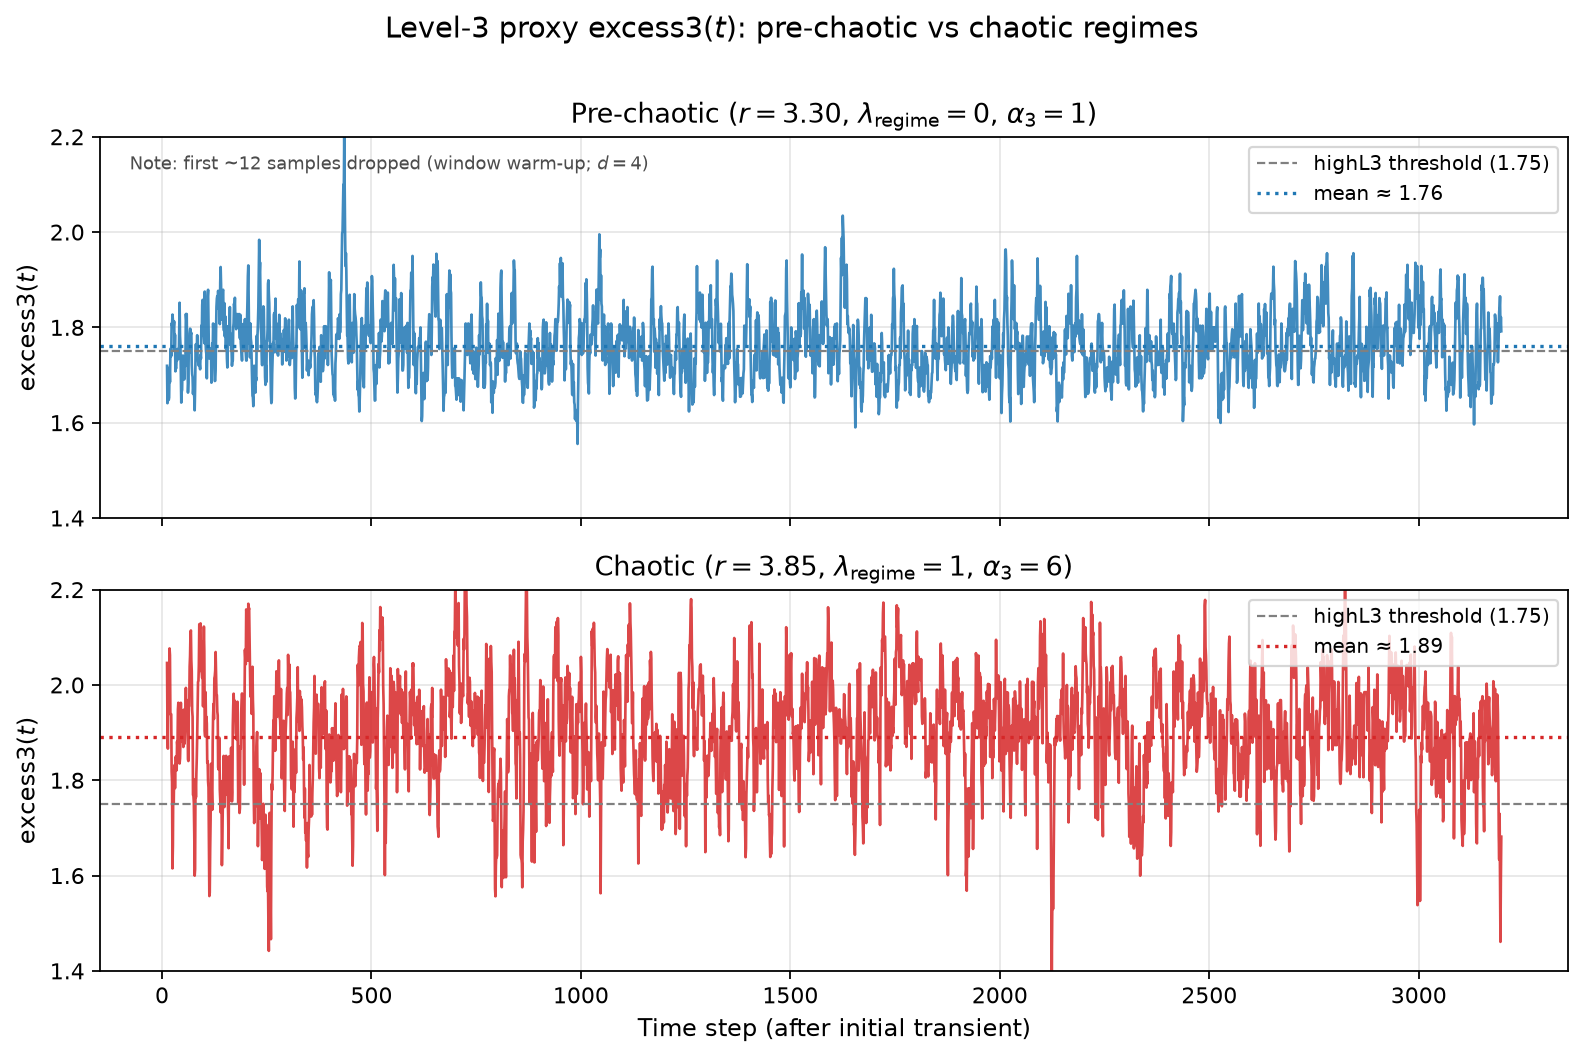
\includegraphics[width=\textwidth]{figures/excess3_pre_vs_chaos.png}
\caption{Level~3 proxy $\mathrm{excess3}(t)$ on representative
realizations of diffusively coupled logistic maps ($d=4$,
$\varepsilon=0.05$). Top: pre-chaotic ($r=3.30$). Bottom: chaotic
($r=3.85$). Dashed line: highL3 threshold $1.75$; dotted line: trajectory
mean. Mean excess3 rises from $\approx 1.76$ to $\approx 1.89$ across the
ensemble (Table~\ref{tab:synthetic}). This is abundance of the proxy,
not $\mathrm{Res}_{\mathrm{pair}}$.}
\label{fig:excess3}
\end{figure}

\begin{figure}[htbp]
\centering
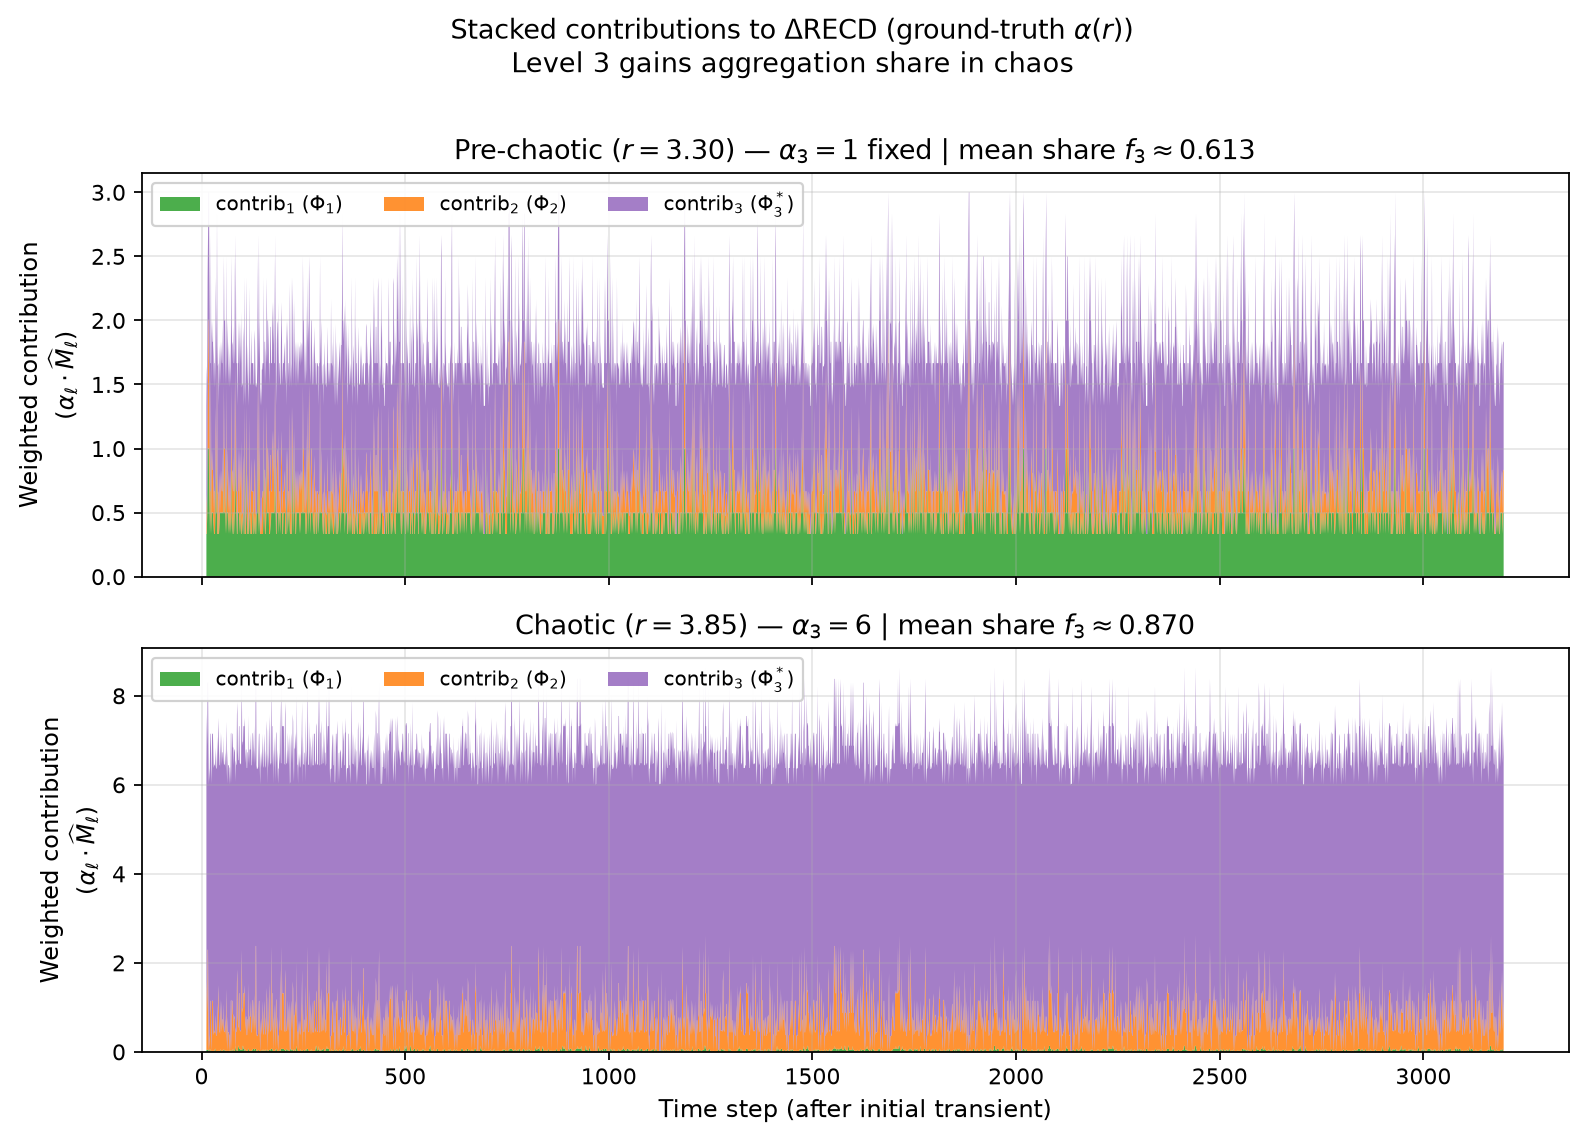
\includegraphics[width=\textwidth]{figures/contribs_stacked_pre_vs_chaos.png}
\caption{Stacked weighted contributions
$\alpha_\ell\Phi_\ell$ to $\Delta\mathrm{RECD}$ under ground-truth regime
labels ($\alpha_3=1$ pre-chaos; $\alpha_3=6$ chaos). Level~3 (top band)
gains aggregation share: mean $f_3$ increases from $\approx 0.613$ to
$\approx 0.870$.}
\label{fig:contribs}
\end{figure}

\begin{figure}[htbp]
\centering
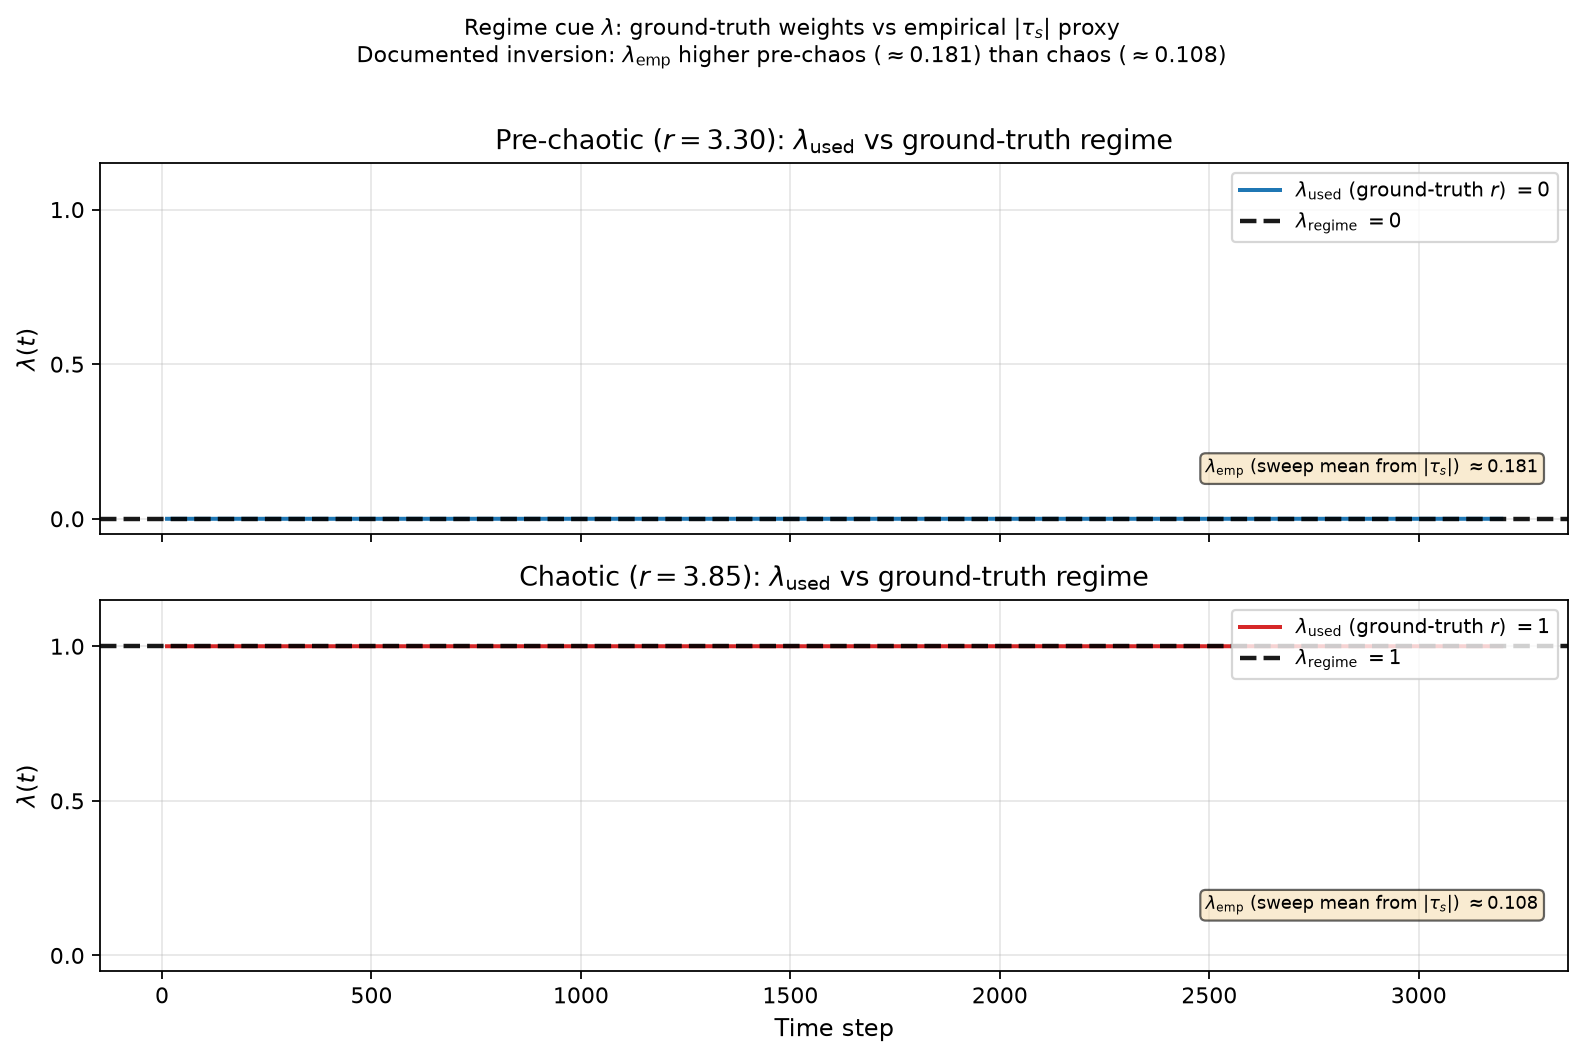
\includegraphics[width=0.95\textwidth]{figures/lambda_emp_vs_regime.png}
\caption{Regime cue $\lambda$: solid curves show $\lambda_{\mathrm{used}}$
from ground-truth $r$ (the weights actually applied in
Figures~\ref{fig:excess3}--\ref{fig:contribs}); dashed lines mark
$\lambda_{\mathrm{regime}}\in\{0,1\}$. Annotated $\lambda_{\mathrm{emp}}$
values are sweep means of the pure $|\tau_s|$-derived proxy, which is
\emph{higher} pre-chaos ($\approx 0.181$) than in chaos ($\approx 0.108$)
on this system---the documented polarity inversion motivating
Appendix~\ref{app:lambda}.}
\label{fig:lambda}
\end{figure}

Raw Level~3 abundance (excess3) increases consistently: mean excess3
rises by approximately $7.5\%$ (Figure~\ref{fig:excess3}), and the
fraction of time spent above the high threshold nearly doubles. Under
intentional reweighting by ground-truth regime, the aggregation share of
$\Delta\mathrm{RECD}$ attributable to Level~3 increases from roughly
$61\%$ to $87\%$ (Figure~\ref{fig:contribs}). Concurrently, mean
$\Phi_1$ and $\Phi_2$ tend to decrease slightly in chaos, as expected
when simple coincidence and clean persistent codes become rarer under
mixing---reinforcing that the excess3 rise is not a trivial rescaling of
Level~1.

Light phase-shuffle surrogates that destroy cross-variable dependence
while preserving marginal spectra \cite{Theiler1992} confirm that, in
the pre-chaotic regime, observed excess3 lies significantly above the
independence null. In chaos the absolute baseline of the excess metric
shifts, so absolute $p$-values against surrogates must be interpreted
jointly with the pre$\to$chaos \emph{delta}, which remains robust. A
secondary methodological finding, highlighted in Figure~\ref{fig:lambda},
is that empirical $|\tau_s|$ on this coupled logistic proxy can be
\emph{higher} in the pre-chaotic synchronized regime than in developed
chaos; hence $\lambda(|\tau_s|)$ requires system-specific calibration
when ground-truth $r$ is unavailable (Appendix~\ref{app:lambda}). This
does not undermine excess3 as a raw Level~3 observable; it disciplines
the use of $\tau_s$-derived weights.

\subsection{Interpretation (binary contrast)}

Within the limits of this synthetic protocol, the data support a
directional hierarchical prediction for the \emph{proxy} abundance
excess3 and, under ground-truth $\lambda(r)$, for the aggregation share
$f_3$. They do not by themselves establish that
$\mathrm{Res}_{\mathrm{pair}}$ tracks excess3 at short windows
(Section~\ref{sec:cascade_sweep}). The RECD is therefore not a
homogeneous counter of coincidences; under a declared engine its
composition tracks both active structure depth and the chosen weights.

\subsection{Dense cascade sweep}
\label{sec:cascade_sweep}

The two-point contrast rejects the coarse null that excess3 abundance is
regime-invariant, but does not locate where along the period-doubling
cascade abundance peaks, nor how it relates to classical EWS or to the
irreducible residual $\mathrm{Res}_{\mathrm{pair}}$.
We therefore recompute the nested pipeline on a dense grid of
$32$ values $r\in[3.10,3.95]$ (densified near
$r_\infty\approx 3.56995$), with $N_{\mathrm{real}}=6$ independent
trajectories of length $T=2200$ after burn-in, and the same
$(d,\varepsilon,\sigma,m,w)$ as above. Reported metrics are mean excess3,
highL3 rate, mean $\mathrm{Res}_{\mathrm{pair}}$ (IPF pairwise maxent,
stride~$8$), mean $|\tau_s|$, and classical variance and lag-1
autocorrelation (channel means).

\begin{figure}[htbp]
\centering
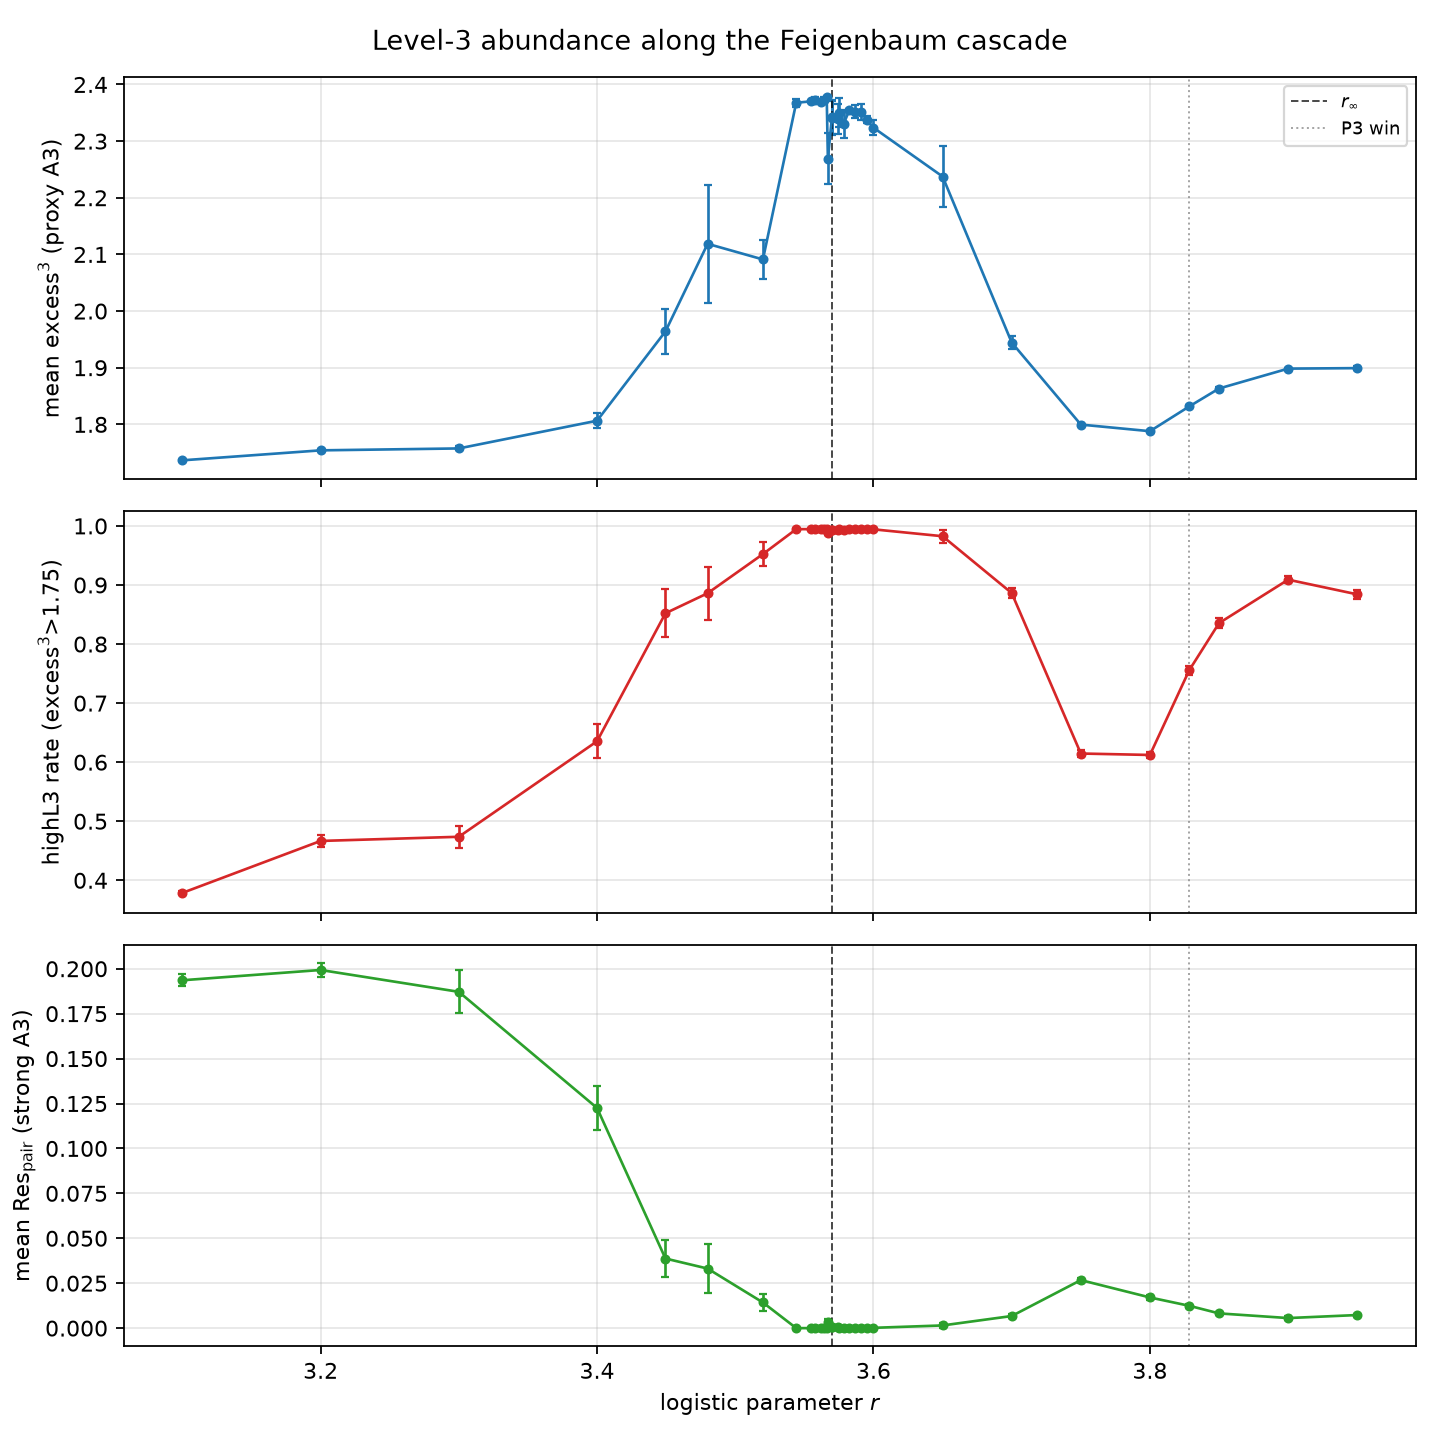
\includegraphics[width=0.98\textwidth]{figures/cascade_A3_vs_r.png}
\caption{Level~3 abundance along the Feigenbaum cascade (coupled logistic
maps, $d=4$, $\varepsilon=0.05$). Top: mean excess3 (proxy $A_3$).
Middle: highL3 rate. Bottom: mean $\mathrm{Res}_{\mathrm{pair}}$
(irreducible residual). Vertical dashed line: $r_\infty$; dotted:
period-3 window onset. Error bars: SEM across realizations.
excess3/highL3 rise from period-$2$ stations into the accumulation band;
the proxy maximum lies near $r_\infty$, not in deep chaos. The bottom
panel uses the dense-sweep window $w=13$; under that protocol
$\mathrm{Res}_{\mathrm{pair}}$ appears highest in low-period stations
(Fig.~\ref{fig:res_diag} shows the window-length correction). The proxy
and the irreducible residual are not interchangeable.}
\label{fig:cascade_A3}
\end{figure}

\begin{figure}[htbp]
\centering
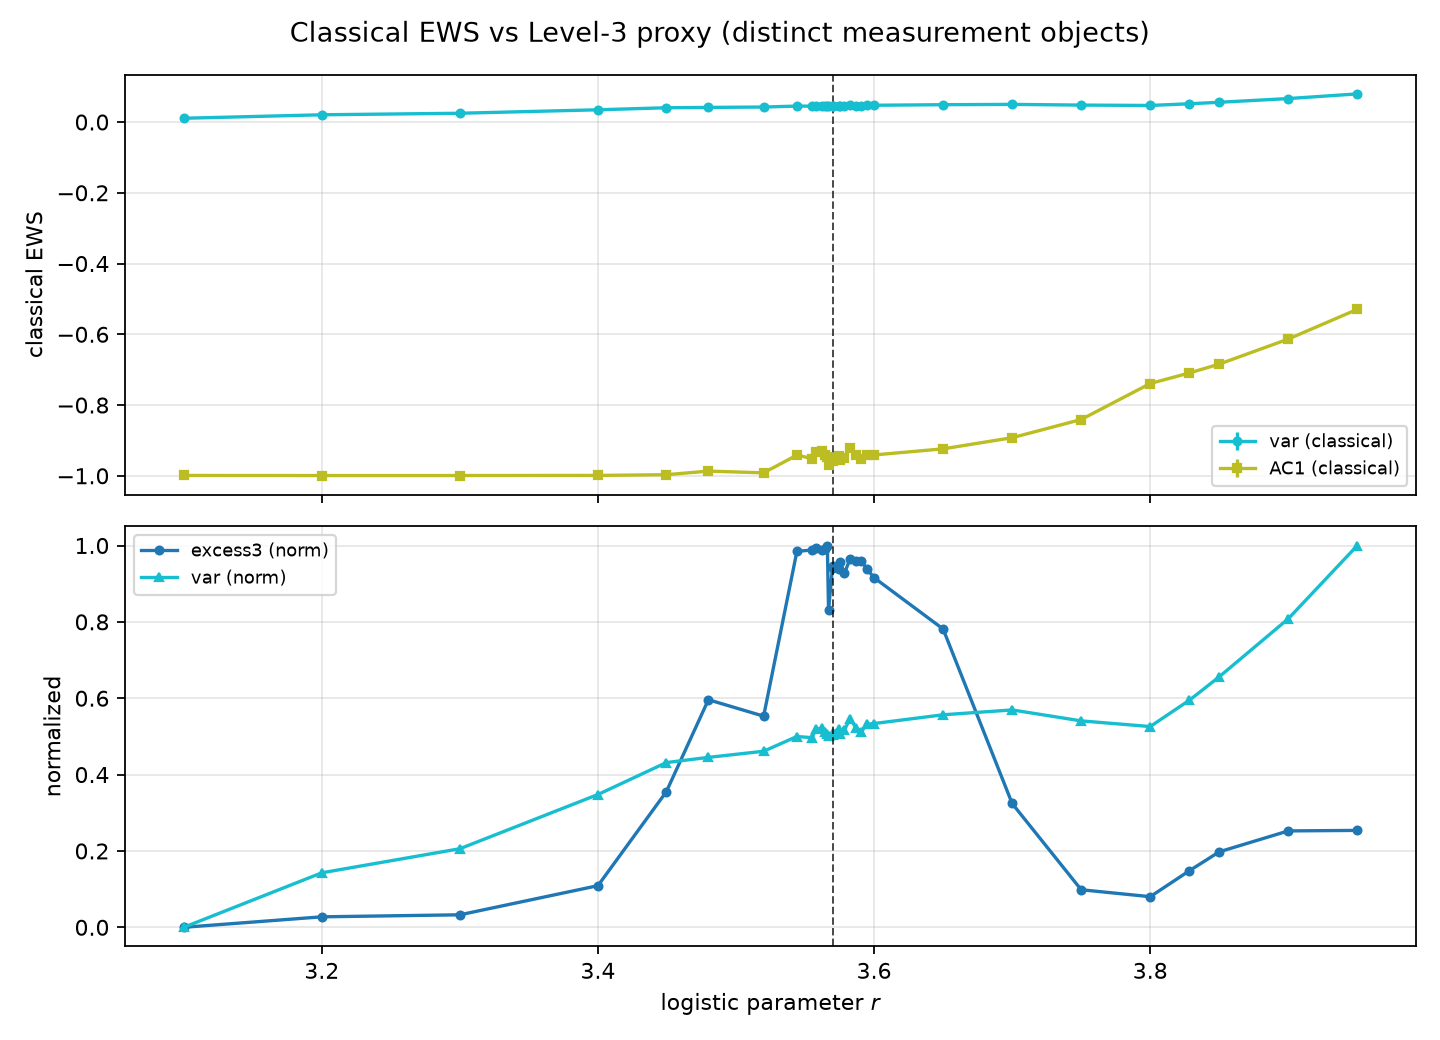
\includegraphics[width=0.98\textwidth]{figures/cascade_ews_vs_A3.png}
\caption{Classical EWS versus Level~3 proxy along the same $r$-grid.
Top: channel-mean variance and lag-1 autocorrelation. Bottom: shapes of
mean excess3 and variance after separate min--max normalization.
Normalized variance does not reproduce the excess3 profile
($\mathrm{corr}_r\approx 0.21$), consistent with the separation of
measurement objects in Section~\ref{sec:chaos}.}
\label{fig:cascade_ews}
\end{figure}

Principal numerical findings on this ensemble are as follows
(synthetic evidence, not analytic theorems):
\begin{enumerate}[leftmargin=*,itemsep=2pt]
  \item \textbf{Coarse mono for the proxy.}
  At the reference stations $r=3.30\to 3.85$, mean excess3 rises
  ($1.76\to 1.86$) and highL3 nearly doubles ($0.47\to 0.84$), matching
  Table~\ref{tab:synthetic} directionally under the denser protocol.
  \item \textbf{Peak location of the proxy.}
  \emph{Observation (result of the suite).} Maximum mean excess3 on the
  grid is near pre-accumulation ($r\approx 3.566$, excess3$\approx 2.38$),
  not at developed chaos. Developed chaos retains elevated highL3 rates
  but intermediate mean excess3. This is a robust synthetic fact on the
  present ensemble.
  \emph{Working hypothesis (not a result).} We tentatively interpret the
  peak as few-state high-period joints near $r_\infty$ (non-product
  support elevating Surp and, when pairwise summaries under-explain TC,
  Syn) versus broader mixing in deep chaos (which can dilute the hybrid
  scores even when $\mathrm{Res}_{\mathrm{pair}}$ at adequate window length
  remains large). The window diagnosis below is \emph{consistent with}
  this hypothesis but does not establish it. A controlled limit of
  $(\mathrm{Syn},\mathrm{Surp},\mathrm{Res}_{\mathrm{pair}})$ along the
  cascade remains future work.
  \item \textbf{Irreducible residual and window length.}
  Under the dense-sweep protocol ($w=13$), $\mathrm{Res}_{\mathrm{pair}}$
  appears largest in period-$2$ stations ($\approx 0.20$) and near zero
  in chaos. A window-length, alphabet-support, and IPF diagnostic shows
  that this is largely an estimator effect: at $r=3.85$, mean
  $\mathrm{Res}_{\mathrm{pair}}$ rises from $\approx 0.009$ ($w=13$) to
  $\approx 1.26$ ($w=104$) and $\approx 0.45$ on a long contiguous
  block, while the IPF procedure converges in all stations. Near
  $r_\infty$ the residual remains low even at long $w$ (few-state
  high-period joint, nearly pairwise-explainable). With adequate $w$,
  the coarse ordering
  $\mathrm{Res}(\mathrm{chaos})>\mathrm{Res}(\mathrm{period\text{-}2})$
  is restored. Claims of the irreducible residual should still separate
  the proxy excess3 from $\mathrm{Res}_{\mathrm{pair}}$ and report the
  window length.
  \item \textbf{Non-triviality vs $|\tau_s|$ and variance.}
  Across $r$, $\mathrm{corr}(\mathrm{excess3},|\tau_s|)\approx 0.27$ and
  $\mathrm{corr}(\mathrm{excess3},\mathrm{var})\approx 0.21$. Systemic Tau
  and nested RECD answer dual questions; classical EWS answer a third.
\end{enumerate}

\begin{figure}[htbp]
\centering
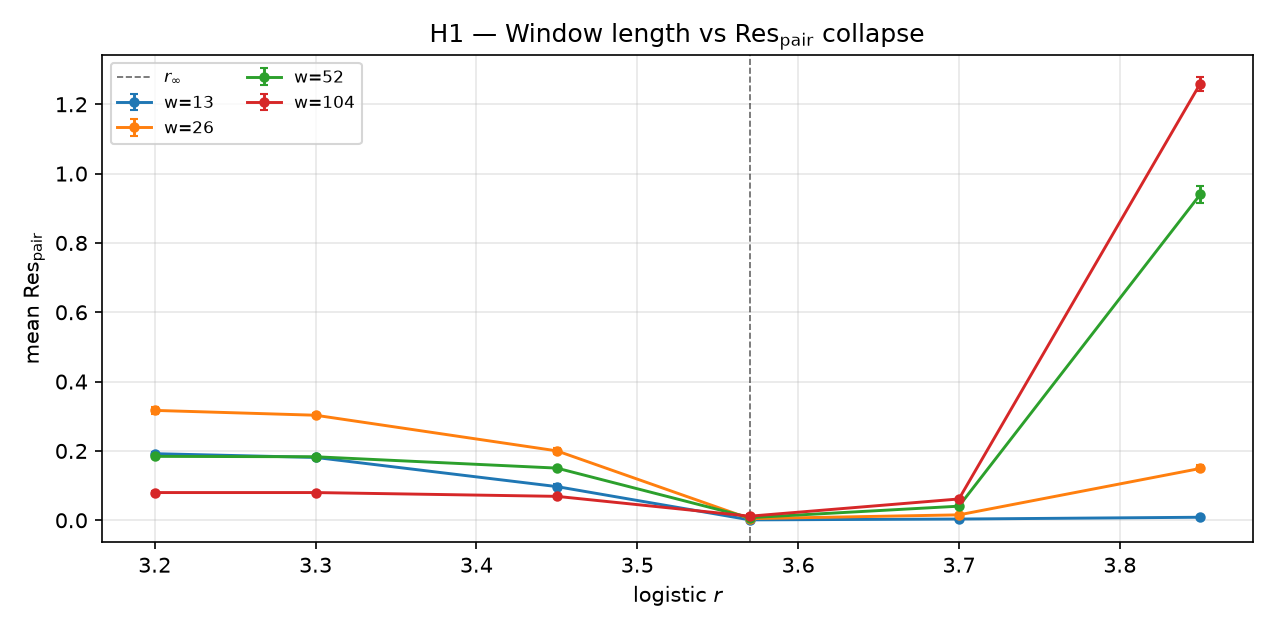
\includegraphics[width=0.98\textwidth]{figures/res_pair_diag_window.png}
\caption{Window-length diagnosis of $\mathrm{Res}_{\mathrm{pair}}$ at
cascade stations. Short windows ($w=13$) suppress the residual in
developed chaos; long windows restore a large residual there, while near
$r_\infty$ the residual remains close to zero. The elevated period-$2$
value at $w=13$ is largely short-window inflation relative to the
long-block estimate.}
\label{fig:res_diag}
\end{figure}

Full numerical tables, companion panels (variability of excess3 and
$|\tau_s|$; $\Phi_1$/$\Phi_2$/$f_3$; residual diagnostics), and
reproducible scripts are provided with the supplemental materials.
The algorithmic implementation is the open \texttt{nested-recd}
library \cite{Padilla2026nested}.

\FloatBarrier
\section{Discussion}
\label{sec:discussion}

\subsection{Conceptual implications}

The framework advanced here casts early warning as a problem of
\emph{hierarchical ordinal structure} rather than of univariate
fluctuation size alone. Systemic Tau supplies a directed scalar of
relational reorganization; nested RECD supplies a depth-resolved,
event-driven clock. Together they answer two distinct but complementary
questions: whether mutual organization is changing, and at what ordinal
depth that change is expressed---provided one keeps structural claims,
estimators, and aggregation weights on separate planes.

First, the sign of $\Delta\tau_s$ is scientifically meaningful rather
than a nuisance: tightening and loosening are different reorganizations,
and both may precede critical transitions depending on the substrate.
Second, the RECD hierarchy makes explicit that not all ordinal events are
equal: coincidence, persistence, and the irreducible residual
$\mathrm{Res}_{\mathrm{pair}}$ occupy different layers of structural
claim, and excess3 is only a proxy for the third. Third, Feigenbaum-motivated scales enter $\lambda$ and the
operational bands as calibrated design structure, not as a derivation of
$\mathrm{Res}_{\mathrm{pair}}$ from Feigenbaum's functional equation.

\subsection{Advantages relative to classical EWS}

Compared with variance and lag-1 autocorrelation, Systemic Tau and RECD
are multivariate by construction, monotone-invariant, and targeted at
coupling geometry. They do not assume a local fixed-point bifurcation,
and they produce a signed relational contrast rather than a one-sided
``rising indicator'' narrative. The Level~3 layer---preferably
$\mathrm{Res}_{\mathrm{pair}}$ when estimable, otherwise excess3 with
explicit caveats---is designed to remain informative when pairwise
synchronization measures saturate or reverse.

\subsection{Relation to neighbouring methodologies}

The framework sits in a neighbourhood of existing ordinal and
information-theoretic tools, but is not reducible to any one of them.

\begin{itemize}[leftmargin=*,itemsep=3pt]
  \item \textbf{Permutation entropy and ordinal networks.}
  Bandt--Pompe encoding and ordinal networks
  \cite{BandtPompe2002,Amigo2010,McCullough2015} provide the symbolic
  substrate of RECD. Permutation entropy compresses the pattern
  distribution of a \emph{single} series into a scalar complexity;
  RECD instead builds a \emph{multivariate hierarchy of conjunctions}
  and an event-driven clock.

  \item \textbf{Recurrence quantification analysis (RQA).}
  RQA quantifies recurrence structure in reconstructed phase space
  \cite{Marwan2007}. RECD is related in spirit---both care about
  returns of structure---but operates in ordinal symbol space with an
  explicit three-level nesting and a coupling to $\tau_s$.

  \item \textbf{Transfer entropy and PID.}
  Transfer entropy measures directed information flow
  \cite{Schreiber2000}; partial information decomposition isolates
  synergistic atoms \cite{Williams2010,Lizier2014}. Our Level~3 claim
  object is the irreducible residual $\mathrm{Res}_{\mathrm{pair}}$;
  excess3 is a simple, falsifiable proxy, not a full PID lattice.
  Natural extensions replace \eqref{eq:excess3} by
  $\mathrm{Res}_{\mathrm{pair}}$ or by an axiomatic PID synergy atom when
  estimators permit.

  \item \textbf{Topological data analysis (TDA).}
  Persistent homology tracks multiscale topological features of point
  clouds \cite{Carlsson2009}. Systemic Tau is ``topological'' only in
  the weak sense of rank geometry; it does not compute barcodes. Hybrid
  pipelines that feed ordinal cores into TDA functors are an open
  direction.
\end{itemize}

\subsection{Limitations}

Several limitations must be stated clearly.

\begin{enumerate}[leftmargin=*,itemsep=2pt]
  \item \textbf{Proxy dependence of Level~3 (central).}
  The proxy excess3 is a hybrid heuristic and is not the irreducible
  residual $\mathrm{Res}_{\mathrm{pair}}$. It can rise under pure pairwise
  (common-driver) geometries via the Surp term; it can agree with
  $\mathrm{Res}_{\mathrm{pair}}$ on XOR-type higher-order joints. The
  coefficients $(0.6,0.4)$ fix a hybrid class a priori
  (Section~\ref{sec:level3}), not a free fit. Alternative estimators
  (pairwise maxent / IPF, PID atoms) may shift quantitative thresholds
  even when qualitative regime contrasts persist. Claims of the
  irreducible residual should name $\mathrm{Res}_{\mathrm{pair}}$ and the
  window length.

  \item \textbf{Calibration of $\lambda$.}
  The map from $|\tau_s|$ to $\lambda$ can invert on some coupled
  systems (Section~\ref{sec:validation}, Figure~\ref{fig:lambda}).
  Regime labels or multi-indicator cues may be required for stable
  aggregation weights; a concrete multi-cue protocol is given in
  Appendix~\ref{app:lambda}. Aggregation shares $f_\ell$ inherit this
  fragility; raw Level~3 abundance does not.

  \item \textbf{Parameter choices.}
  Embedding $(m,\tau)$, persistence $p_{\min}$, windows $W$ and $w$,
  and $\theta_3$ are operational. Sensitivity analysis is mandatory in
  any empirical use; the present paper reports a reference configuration
  used in synthetic tests.

  \item \textbf{Scope of validation.}
  The synthetic protocol uses weakly coupled logistic maps at fixed
  coupling, with a binary contrast and a denser $r$-grid along the
  cascade. It supports directional predictions on proxy abundance
  (excess3) and---under ground-truth $\lambda$---on the aggregation
  share $f_3$; it does not exhaust the bifurcation structure of
  high-dimensional networks \cite{Strogatz2001}, nor prove limit
  theorems for $\mathrm{Res}_{\mathrm{pair}}(r)$ along the full Feigenbaum
  cascade. The excess3 peak near $r_\infty$ is a robust observation; the
  few-state vs.\ mixing account in Section~\ref{sec:cascade_sweep} is a
  working hypothesis only.

  \item \textbf{Aggregation policy, not metaphysics.}
  The aggregation share $f_\ell$ in \eqref{eq:frac} is an axiomatized
  design output, not a unique law of the joint symbol process and not a
  substitute for $\mathrm{Res}_{\mathrm{pair}}$.
\end{enumerate}

\section{Conclusions and Outlook}
\label{sec:conclusions}

We have laid foundations for Systemic Tau and hierarchical ordinal
conjunctions---with nested RECD as the operational discrete clock---as a
dual relational account of critical transitions. Systemic Tau ($\tau_s$) aggregates Kendall-type concordance
across coordinates into a multivariate ordinal measure of coupling,
equipped with Feigenbaum-motivated operational bands and a directed
contrast $\Delta\tau_s$. The RECD constructs an intrinsic discrete clock
from three levels of structural claim---coincidence ($\Phi_1$),
persistent relational structure ($\Phi_2$), and the irreducible residual
beyond pairwise models ($\mathrm{Res}_{\mathrm{pair}}$)---together with a
scalable proxy excess3 that must not be identified with that residual.
Regime-dependent weights $\alpha_\ell(\lambda)$ form an admissible
aggregation policy that can shift the aggregation share of
$\Delta\mathrm{RECD}$ toward deeper layers near chaos; they do not
create Level~3 geometry. In this language, early warning is cast as a
reorganization of hierarchical ordinal structure, not merely a rise in
fluctuation size---with claims, estimators, and aggregation kept distinct.

A controlled synthetic validation on coupled logistic maps supports a
directional prediction for proxy abundance (excess3) and, under
ground-truth $\lambda(r)$, for the aggregation share $f_3$ of
$\Delta\mathrm{RECD}$ from pre-chaotic to chaotic regimes. The same suite
documents window bias for $\mathrm{Res}_{\mathrm{pair}}$, polarity
inversion of $|\tau_s|$-based cues, and a proxy peak near accumulation
(observation) with only a working hypothesis for its geometry. Classical
EWS remain valuable inside their theoretical domain; the present
framework is offered as a complement for high-dimensional, noisy, and
nonstationary systems where relational geometry---and its depth---may
carry a leading signature of criticality.

Promising directions include: (i)~routine estimation of
$\mathrm{Res}_{\mathrm{pair}}$ and head-to-head comparison with excess3 on
XOR versus common-driver synthetics; (ii)~axiomatic PID synergy
estimators in place of the hybrid when feasible; (iii)~extensions beyond
three levels or to multilayer networks; (iv)~multi-cue $\lambda$ as an
incomplete-information estimator of the regime coordinate
(Appendix~\ref{app:lambda}); (v)~limit theorems for proxy abundance and
$\mathrm{Res}_{\mathrm{pair}}$ along the Feigenbaum cascade, including a
proper test of the few-state vs.\ mixing \emph{hypothesis} for the peak
near $r_\infty$, and shared benchmarks against standard CSD suites.
Empirical domains---from epidemiology to network physiology---provide
natural testing grounds. The foundational contribution is a coherent
calculus that keeps proxy and irreducible residual, and abundance and
aggregation share, distinct.

\appendix
\section{Calibration of the regime cue}
\label{app:lambda}

This appendix records an operational protocol for constructing
$\lambda$ when the pure $|\tau_s|$ proxy is unreliable---as documented
for the coupled logistic ensemble of Section~\ref{sec:validation}---while
preserving the design goal that $\lambda$ increase toward chaotic or
high-volatility regimes.

\subsection{Design goal and polarity}

Let $\mathcal{R}_{\mathrm{chaos}}$ denote the set of regimes in which
Level~3 abundance is predicted to rise (developed chaos, strong mixing,
or analogous high-volatility states). The aggregation engine requires
\begin{equation}
\label{eq:lambda-goal}
\mathbb{E}\bigl[\lambda \mid \mathcal{R}_{\mathrm{chaos}}\bigr]
\;>\;
\mathbb{E}\bigl[\lambda \mid \mathcal{R}_{\mathrm{pre}}\bigr],
\end{equation}
so that $\alpha_3(\lambda)$ in \eqref{eq:alphas} elevates rather than
suppresses the Level~3 term in the clock. Equation~\eqref{eq:lambda}
supplies a one-parameter family indexed by polarity $s\in\{+1,-1\}$.
The correct $s$ is \emph{not} universal: it encodes whether the system
desynchronizes ($|\tau_s|$ falls) or remains strongly rank-coupled (or
anti-coupled) as chaos develops.

\paragraph{Polarity diagnostic.}
Given labeled training windows from pre-critical and post-critical (or
pre-chaos / chaos) segments, estimate
$\overline{|\tau_s|}_{\mathrm{pre}}$ and
$\overline{|\tau_s|}_{\mathrm{chaos}}$. Set
\begin{equation}
s
=
\begin{cases}
-1 & \text{if }
\overline{|\tau_s|}_{\mathrm{chaos}}
<\overline{|\tau_s|}_{\mathrm{pre}},\\
+1 & \text{otherwise.}
\end{cases}
\end{equation}
On the $d=4$ logistic proxy of Section~\ref{sec:validation},
$\overline{|\tau_s|}$ is higher pre-chaos than in chaos, so the
diagnostic returns $s=-1$. Figure~\ref{fig:lambda}'s annotated
$\lambda_{\mathrm{emp}}$ values ($\approx 0.181$ pre vs.\
$\approx 0.108$ chaos) correspond to the \emph{uncalibrated}
$s=+1$ template and therefore violate \eqref{eq:lambda-goal}; applying
$s=-1$ restores directional consistency for that proxy. When even a
polarity-corrected $|\tau_s|$ cue remains weak relative to spectral or
recurrence channels, a multi-cue construction is preferred.

\subsection{Multi-cue consensus}

\paragraph{Status.}
The cue $\lambda$ is the regime coordinate of the aggregation engine
$(\lambda,\alpha)$: the scalar that moves $\alpha_\ell$ under depth
monotonicity (Section~\ref{sec:alpha}). With known control parameter one
sets $\lambda=\lambda(r)$. When $r$ is latent, $\lambda$ must be
estimated. A single channel $\lambda_\tau(|\tau_s|)$ fails the design goal
\eqref{eq:lambda-goal} whenever ordinal coupling and chaoticity are not
monotone together (Section~\ref{sec:validation})---a limitation of that
channel as a regime statistic, not of Systemic Tau as a relational
observable.

Multi-cue $\lambda$ is therefore an incomplete-information estimator of
the same coordinate: a small convex consensus of independent regime
signatures standard in nonlinear time series (rank coupling, spectral
complexity, recurrence). It is a design object for the aggregation plane,
not a dynamical law of $S_t$ and not a substitute for
$\mathrm{Res}_{\mathrm{pair}}$ or proxy abundance. Naturalness criteria:
channels probe distinct aspects of the transition; no channel dominates
$\alpha_3$ by circular construction; convex weights are fixed on a
labeled holdout, not tuned to maximize $f_3$ on the test set.

\paragraph{Construction.}
Define a small set of normalized cues $c_j(t)\in[0,1]$, each increasing
with estimated chaoticity after its own polarity calibration:
\begin{itemize}[leftmargin=*,itemsep=2pt]
  \item $c_\tau$: monotone transform of $|\tau_s|$ with polarity $s$ as
  above (e.g.\ a logistic map of
  $s\,(|\tau_s|-\tau_{\mathrm{ch}})/\tau_{\mathrm{ch}}$ onto $[0,1]$);
  \item $c_{\mathrm{spec}}$: spectral broadbandness (fraction of power
  above a mid-band cutoff, or spectral entropy);
  \item $c_{\mathrm{rqa}}$: recurrence irregularity (e.g.\ $1-\mathrm{DET}$
  or laminarity deficit from recurrence quantification
  \cite{Marwan2007});
  \item $c_{\mathrm{L3}}$: raw Level~3 \emph{abundance} (windowed mean
  excess3, min--max normalized on a reference epoch), used only as a
  \emph{slow} cue with small weight to avoid circular domination of
  $\alpha_3$ by the quantity it reweights.
\end{itemize}
The consensus cue is the convex combination
\begin{equation}
\label{eq:lambda-multi}
\lambda_{\mathrm{multi}}(t)
=
\Bigl(\sum_{j\in\mathcal{J}} w_j\,c_j(t)\Bigr)
\cdot
\bigl(1+\gamma\log\delta\bigr),
\qquad
w_j\geq 0,\quad
\sum_{j\in\mathcal{J}} w_j=1,
\end{equation}
with default equal weights on $\{c_\tau,c_{\mathrm{spec}},c_{\mathrm{rqa}}\}$
and optional small weight on $c_{\mathrm{L3}}$ ($w_{\mathrm{L3}}\leq 0.15$)
when independent spectral/RQA channels are unavailable. The Feigenbaum
prefactor $(1+\gamma\log\delta)$ is retained for continuity with
\eqref{eq:lambda} (role $\delta_{\mathrm{cue}}$ only).

\subsection{Fallback hierarchy}

In applications we recommend the following precedence:
\begin{enumerate}[leftmargin=*,itemsep=2pt]
  \item \textbf{Ground-truth control} $r$ (or known regime labels): set
  $\lambda=\lambda(r)$ monotone (as in Section~\ref{sec:validation}).
  \item \textbf{Multi-cue consensus} \eqref{eq:lambda-multi} with
  polarity diagnostics on a labeled calibration segment.
  \item \textbf{Single-proxy} $\lambda_\tau$ of \eqref{eq:lambda} only
  after verifying \eqref{eq:lambda-goal} on held-out labeled windows.
  \item \textbf{Unweighted RECD} ($\alpha_\ell\equiv 1$): report raw
  $\Phi_\ell$ and excess3 contrasts without aggregation reweighting when
  no reliable cue exists.
\end{enumerate}
This hierarchy separates two claims that the main text keeps distinct:
(i)~Level~3 \emph{abundance} (excess3, highL3, or
$\mathrm{Res}_{\mathrm{pair}}$) is a raw hierarchical observable and does
not require $\lambda$; (ii)~Level~3 \emph{aggregation share} $f_3$ under
$\alpha_\ell(\lambda)$ is a regime-aware construct whose validity
inherits from the quality of $\lambda$. The synthetic validation of
Section~\ref{sec:validation} tests (i) unconditionally and (ii) under
ground-truth $\lambda(r)$, while Figure~\ref{fig:lambda} and the
present appendix document why (ii) must not be claimed from an
uncalibrated $|\tau_s|$ proxy on every system.

\section*{Acknowledgments}
The author thanks collaborators and open-source contributors to the
\texttt{systemictau} ecosystem, and acknowledges the broader complex-systems
community whose work on early warning signals, ordinal patterns, and
Feigenbaum universality made the present synthesis possible.

\bibliographystyle{plainnat}
\bibliography{references}

\end{document}
